\id{МРНТИ 31.01.05}

{\bfseries ИЗУЧЕНИЕ СПОСОБОВ ОПРЕСНЕНИЯ МОРСКОЙ ВОДЫ МЕТОДОМ ПРЯМОГО
ОСМОСА}

{\bfseries \textsuperscript{1}Қ.А. Куртибай}\textsuperscript{\envelope }{\bfseries ,
\textsuperscript{1}Ә. Қаппасұлы, \textsuperscript{2}Е.Е. Жатканбаев,
\textsuperscript{3}Ж.К. Жатканбаева,}

{\bfseries \textsuperscript{1}М.Б. Султанкул, \textsuperscript{1}Н.Б.
Молдагулова, \textsuperscript{1}А.Ә. Үсенова,}
{\bfseries \textsuperscript{1}Г.А. Данлыбаева}

\textsuperscript{1} ТОО «Научно-производственный центр экологической и
промышленной биотехнологии», Астана, Казахстан,

\textsuperscript{2} Казахский университет технологии и бизнеса имени К.
Кулажанова, Астана, Казахстан,

\textsuperscript{3} Евразийский Национальный Университет имени Л.Н.
Гумилёва, Астана, Казахстан

\textsuperscript{\envelope }Корреспондент-автор: kurtibayqb@gmail.com

В статье рассматриваются методы опреснения морской соленой воды методом
прямого осмоса с использованием различных вытяжных растворов с высоким
осмотическим давлением при разных концентрациях. Исследование охватывает
применение хлорида натрия, сахарозы и бикарбоната аммония. В качестве
исходных растворов использовались морская вода из Каспийского и
Средиземного морей, а также растворы хлорида натрия с концентрацией,
соответствующей солёности морской воды.

Результаты экспериментов подтвердили прямую зависимость между
концентрацией вытяжного раствора и потоком воды. Высокая концентрация
вытяжного раствора приводит к повышению осмотического давления, что
способствует увеличению потока воды через мембрану. Максимальный поток
воды был зафиксирован на первых сутках эксперимента. При использовании
хлорида натрия в концентрациях 9\%, 18\% и 25\% для опреснения воды
Средиземного моря поток воды через мембрану составил 20,29 л·м⁻²·ч⁻¹,
55,7 л·м⁻²·ч⁻¹ и 81,12 л·м⁻²·ч⁻¹ соответственно. В сравнении с обратным
осмосом, который имеет производительность 7,5 л·м⁻²·ч⁻¹/кПа, метод
прямого осмоса демонстрирует значительное преимущество. Объем полученной
чистой воды при концентрациях 9\%, 18\% и 25\% составил 272 см³, 647 см³
и 741 см³ соответственно. Таким образом, можно сделать вывод, что с
увеличением массовой концентрации раствора хлорида натрия используемый в
качестве вытяжного раствора объем получаемой чистой воды также
увеличивается. При опреснении воды Каспийского моря максимальный поток
воды с 25\%-ным вытяжным раствором был достигнут в первый день
эксперимента и составил 91,0 л·м⁻²·ч⁻¹, объем чистой воды после
регенерации --- 579 см³. Эксперименты с сахарозой показали, что поток
воды возрастает с увеличением концентрации вытяжного раствора,
максимальный поток воды достиг 31,33 л·м⁻²·ч⁻¹ при использовании 70\%
сахарозы. Объем чистой воды после регенерации составил 105 см³. Способ
опреснения морской воды с использованием бикарбоната аммония оказался
наиболее эффективным и экономичски целесообразным, обеспечив
максимальный поток воды 71,5 л·м⁻²·ч⁻¹ при концентрации вытяжного
раствора 3,846 моль/л. Регенерация воды осуществлялась термической
обработкой раствора в интервале температур 36-70 °С, при этом получено
556 см³ чистой воды, не включая объем воды, использованной для
приготовления раствора.

Полученные результаты подтверждают значительный потенциал прямого осмоса
для эффективного опреснения соленых вод, что имеет важное значение для
решения проблемы доступа к чистой воде в мире, включая Казахстан.

{\bfseries Ключевые слова:} прямой осмос, вытяжной раствор, опреснение,
морская вода, осмотическое давление, поток воды.

{\bfseries ТІКЕЛЕЙ ОСМОС ӘДІСІ АРҚЫЛЫ ТЕҢІЗ СУЫН ТҰЩЫЛАНДЫРУ ТӘСІЛДЕРІН
ЗЕРТТЕУ}

{\bfseries \textsuperscript{1}Қ.А. Куртибай}\textsuperscript{\envelope }{\bfseries ,
\textsuperscript{1}Ә. Қаппасұлы, \textsuperscript{2}Е.Е. Жатканбаев,
\textsuperscript{3}Ж.К. Жатканбаева,}

{\bfseries \textsuperscript{1}М.Б. Султанкул, \textsuperscript{1}Н.Б.
Молдагулова, \textsuperscript{1}А.Ә. Үсенова, \textsuperscript{1}Г.А.
Данлыбаева}

\textsuperscript{1} «Экологиялық және өнеркәсіптік биотехнологияның
ғылыми-өндірістік орталығы» ЖШС, Астана, Қазақстан,

\textsuperscript{2} Қ. Құлажанов атындағы Қазақ технология және бизнес
университеті, Астана, Қазақстан,

\textsuperscript{3} Л.Н. Гумилев атындағы Еуразия Ұлттық Университеті,
Астана, Қазақстан,

e-mail: kurtibayqb@gmail.com

Мақалада әртүрлі концентрациялардағы жоғары осмостық қысымы бар әртүрлі
тартқыш ерітінділерін пайдалана отырып, теңіздің тұзды суын тікелей
осмос әдісімен тұщыландыру тәсілдері қарастырылады. Зерттеуде натрий
хлориді, сахароза және аммоний тұздары сияқты әртүрлі тартқыш
ерітінділерді пайдалана отырып, тікелей осмос әдісімен тұщыландыру
қарастырды. Тікелей осмос әдісімен суды тұщыландыру бойынша зерттеу
барысында бастапқы ерітінді ретінде Каспий және Жерорта теңіздерінің
теңіз суы, сондай-ақ теңіз суының тұздылығына сәйкес келетін
концентрациядағы натрий хлориді ерітінділері пайдаланылды.

Эксперимент нәтижелері тартқыш ерітіндінің концентрациясы мен су ағыны
арасындағы тікелей байланысты растады. Тартқыш ерітіндінің жоғары
концентрациясы осмостық қысымның жоғарылауына әкелетіні анықталды, бұл
мембрана арқылы судың үлкен ағынын ынталандырады. Барлық
эксперименттерде максималды су ағыны тәжірибенің алғашқы күндерінде
тіркелді. Жерорта теңізінің суын тұщыландыру үшін 9\%, 18\% және 25\%
концентрациядағы натрий хлориді ерітінділерін қолданғанда, мембрана
арқылы су ағыны сәйкесінше 20,29 л·м⁻²·сағ⁻¹, 55,7 л·м⁻²·сағ⁻¹ және
81,12 л·м⁻²·сағ⁻¹ болды. Өнімділігі 7,5 л·м-2 * сағ⁻1/кПа болатын кері
осмоспен салыстырғанда, тікелей осмос әдісі айтарлықтай артықшылықты
көрсетеді. Натрий хлоридінің 9\%, 18\% және 25\% концентрацияларында
алынған таза судың көлемі сәйкесінше 272 см³, 647 см³ және 741 см³
болды. Осылайша, тартқыш ерітінді ретінде қолданылатын натрий хлориді
ерітіндісінің массалық концентрациясы ұлғайған сайын, таза судың
алынатын көлемі де ұлғаятыны туралы қорытынды жасауға болады. Каспий
теңізінің суын тұщыландыру кезінде 25\%-дық тартқыш ерітіндімен
максималды су ағыны эксперименттің бірінші күнінде 91,0 л·м⁻²·сағ⁻¹
тіркелді, регенерациядан кейінгі таза судың көлемі 579 см³ құрады.
Сахарозамен жүргізілген эксперименттерде тартқыш ерітіндінің
концентрациясы артқан сайын су ағынының да ұлғаятыны байқалды, 70\%
сахароза қолданған кезде максималды су ағыны 31,33 л·м⁻²·сағ⁻¹ болды, ал
регенерациядан кейінгі таза судың көлемі 105 см³ құрады. Аммоний
бикарбонатын қолдану арқылы теңіз суын тұщыландыру тәсілі ең тиімді және
экономикалық тұрғыдан орынды болды, 3,846 моль/л концентрациядағы
тартқыш ерітіндімен максималды су ағыны 71,5 л·м⁻²·сағ⁻¹ құрады. Судың
регенерациясы ерітіндіні 36-70 °С температуралық интервалда термиялық
өңдеумен жүзеге асырылды, бұл ретте ерітіндіні дайындау үшін
пайдаланылған судың көлемін қоспағанда, 556 см\textsuperscript{3} таза
су алынды.

Алынған нәтижелер тұзды суларды тиімді тұщыландыру үшін тікелей осмостың
елеулі әлеуетін растайды, бұл Қазақстанды қоса алғанда, әлемдегі таза
суға қол жеткізу проблемасын шешу үшін маңызды мәнге ие.

{\bfseries Түйін сөздер:} тікелей осмос, тартқыш ерітінді, тұщыландыру,
теңіз суы, осмостық қысым, су ағыны.

{\bfseries STUDY OF SEAWATER DESALINATION BY FORWARD OSMOSIS METHOD}

{\bfseries \textsuperscript{1}K.A. Kurtibay\textsuperscript{\envelope },
\textsuperscript{1}A. Kappassuly, \textsuperscript{2}Ye.Ye.
Zhatkanbayev, \textsuperscript{3}Zh.K. Zhatkanbayeva,}

{\bfseries \textsuperscript{1}M.B. Sultankul, \textsuperscript{1}N.B.
Moldagulova, \textsuperscript{1}A.A. Ussenova, \textsuperscript{1}G.A.
Danlybayeva}

\textsuperscript{1} «Scientific and Production Center of Ecological and
Industrial Biotechnology» LLP, Astana, Kazakhstan,

\textsuperscript{2} Kazakh University of Technology and Business named
after K. Kulazhanov, Astana, Kazakhstan,

\textsuperscript{3} L.N. Gumilyev Eurasian National University, Astana,
Kazakhstan,

e-mail: kurtibayqb@gmail.com

The article deals with the methods of desalination of sea salt water by
forward osmosis using different draw solutions with high osmotic
pressure at different concentrations. The study covers the use of sodium
chloride, sucrose and ammonium bicarbonate. Seawater from the Caspian
and Mediterranean seas, as well as sodium chloride solutions with
concentrations corresponding to the salinity of seawater were used as
starting solutions.

The experimental results confirmed a direct correlation between the
concentration of the draw solution and the water flow. High
concentration of the draw solution leads to an increase in osmotic
pressure, which favours an increase in water flux through the membrane.
The maximum water flux was recorded on the first day of the experiment.
Using sodium chloride at concentrations of 9\%, 18\% and 25\% for
Mediterranean desalination, the water flux through the membrane was
20.29 l·m⁻²·h⁻¹, 55.7 l·m⁻²·h⁻¹ and 81.12 l·m⁻²·h⁻¹, respectively.
Compared to reverse osmosis, which has a capacity of 7.5 l·m⁻²·h⁻¹/kPa,
the forward osmosis method shows a significant advantage. The volume of
pure water obtained at concentrations of 9\%, 18\% and 25\% was 272 cm³,
647 cm³ and 741 cm³ respectively. Thus, it can be concluded that as the
mass concentration of sodium chloride solution increases, the volume of
pure water obtained also increases with increasing mass concentration of
sodium chloride solution used as a draw solution. In desalination of
Caspian Sea water, the maximum water flux with 25\% draw solution was
reached on the first day of the experiment and was 91.0 l·m⁻²·h⁻¹, the
volume of pure water after regeneration was 579 cm³. Experiments with
sucrose showed that the water flux increased with increasing
concentration of extraction solution, the maximum water flux reached
31.33 l·m⁻²·h⁻¹ when 70\% sucrose was used. The volume of pure water
after regeneration was 105 cm³. The method of seawater desalination
using ammonium bicarbonate proved to be the most effective and
economically feasible, providing a maximum water flux of 71.5 l·m⁻²·h⁻¹
at a draw solution concentration of 3.846 mol/l. Water regeneration was
carried out by thermal treatment of the solution in the temperature
range of 36-70 °C, and 556 cm³ of pure water was obtained, not including
the volume of water used for solution preparation.

The results obtained confirm the significant potential of forward
osmosis for effective desalination of saline water, which is important
for solving the problem of access to clean water in the world, including
Kazakhstan.

{\bfseries Keywords:} forward osmosis, draw solution, desalination,
seawater, osmotic pressure, water flux.

{\bfseries Введение.} Вода, независимо от ее состояния, является ключевым
элементом, через который климат влияет на человека, окружающую среду и
социальное благополучие. Она играет фундаментальную роль в формировании
условий жизни, поддерживает жизненные процессы на планете и обеспечивает
основу для экономического и социального развития.

Цели устойчивого развития (ЦУР) Организации Объединенных Наций (ООН),
установленные 15 сентября 2015 года под названием «Преобразование нашего
мира: Повестка дня в области устойчивого развития на период до 2030
года», имеют решающее значение в контексте нехватки воды. По оценкам
экспертов по водным ресурсам казахстанского офиса ПРООН, в нашей стране
начинает складываться дефицит водных ресурсов, и, по предварительным
прогнозам, к 2040 году этот дефицит может достичь 50\% от общей
потребности. Поскольку питьевая вода необходима практически всем
отраслям экономики, ее нехватка в регионах страны может привести к
снижению ВВП Казахстана примерно на 6 \% к 2050 году, что представляет
собой серьезный вызов для развития национальной экономики {[}1{]}.
Растущий дефицит водных ресурсов представляет собой еще одну из угроз,
стоящих перед человечеством. По прогнозам, к 2050 году до половины
городского населения мира может столкнуться с нехваткой воды {[}2{]}. По
оценкам, на Земле имеется 1 386 000 000 000 000 км\textsuperscript{3}
воды, которая покрывает около 70\% нашей планеты. Вода существует в трех
основных формах: соленая вода (97,5\%), пресная вода (0,5\%) и другие
формы, такие как ледниковый лед/снег (2,5\%) {[}3{]}. Учитывая, что
спрос на воду будет продолжать расти вместе с ростом населения планеты,
ожидается, что научные и инженерные решения сыграют решающую роль в
решении некоторых водных проблем на планете {[}4{]}. Развитие нескольких
технологий очистки воды фактически сделало большинство источников воды
безопасными для различных целей, включая воду из нетрадиционных
источников.

В последнее время прямой осмос как новая мембранная технология
привлекает к себе огромное внимание в связи с ее использованием для
очистки воды {[}5{]}. Прямой осмос --- это процесс, при котором вода
перемещается через полупроницаемую мембрану под воздействием разницы
осмотического давления {[}6{]}. В ходе прямого осмоса полупроницаемая
мембрана разделяет два раствора с разной концентрацией.
Высококонцентрированный раствор называется «вытяжным» (draw), а
низкоконцентрированный -- «исходным» (feed). Это объясняется тем, что в
процессе раствор с высокой соленостью «вытягивает» воду из раствора с
низкой соленостью, который в свою очередь «подаёт» воду в процесс
{[}7{]}. Различие в осмотическом давлении между двумя растворами
является движущей силой, которая приводит к миграции воды с более
разбавленной стороны на сторону с более концентрированным раствором
{[}8{]}. В случае обратного осмоса на сторону с более разбавленным
раствором оказывается давление, превышающее осмотическое давление, что
заставляет воду перемещаться от концентрированной стороны к менее
концентрированной.

Согласно исследованию Suwaileh W. A и коллег {[}9{]}, несмотря на явные
плюсы, прямой осмос сталкивается с определенными проблемами, что
ограничивает его использование. Признание и понимание этих ограничений
играют важную роль в оптимизации использования данной технологии. Одной
из ключевых проблем является поиск подходящих мембран, обеспечивающих
высокий объем перерабатываемой воды при минимальном обратном потоке
соли.

Среди этих преимуществ возможность эксплуатации прямого осмоса при
низких затратах, поскольку вода движется через мембрану от исходного
раствора к раствору за счет градиента осмотического давления, а не
гидравлического давления. Это способствует тому, что процесс прямого
осмоса обеспечивает не только низкое энергопотребление системы и высокую
адаптивность, но и высокий поток воды и меньшее загрязнение мембраны за
счет отбраковки широкого спектра загрязняющих веществ {[}10{]}. Как
следствие, для прямого осмоса требуется высококонцентрированный раствор
для вытяжки, чтобы вызвать движущую силу разделения, и, таким образом,
молекулы воды начнут переходить из исходного материала в раствор для
извлечения {[}11,12{]}. В процессе этого процесса большинство
растворенных молекул или многозарядные ионы, уже присутствующие в
питательной воде, задерживаются мембраной. По мере того, как вода
продолжает проходить через мембрану, вытяжной раствор становится более
разбавленным, что приводит к снижению осмотического давления
вытягивающего раствора, в то время как осмотическое давление исходного
раствора увеличивается, пока не будет достигнуто точки осмотического
равновесия. Это определит конечную концентрацию разбавленного
вытягивающего раствора, который требует дополнительного процесса для
удаления растворенного вещества и получения чистой воды, поскольку
продукт (т.е. разбавленный вытяжной раствор) не может потребляться
непосредственно в виде пресной воды {[}12{]}. Таким образом, мембранный
прямой осмос и раствор для вытяжки, безусловно, являются сердцем системы
прямого осмоса (FO-системы) и играют важную роль в продвижении прямого
осмоса к коммерциализации.

Вытяжной раствор является фундаментальным компонентом процесса прямого
осмоса и источником его движущей силы. Он представляет собой
концентрированный раствор с более высоким осмотическим давлением для
извлечения воды из сырья через мембрану. Развитие технологии прямого
осмоса зависит от наличия подходящего вытяжного раствора. В последнее
время были предприняты значительные усилия для разработки нового
вытяжного раствора, который соответствует следующим критериям: высокая
проницаемость для воды, низкая обратная диффузия солей, минимальная
вязкость, устойчивость к загрязнению, химическая стабильность и
совместимость с мембраной, отсутствие токсичности, нейтральный pH,
низкая стоимость и быстрое восстановление разбавленного раствора с
низким энергопотреблением {[}13,14,15{]}.

Одно из ранних исследований, касающихся применения прямого осмоса для
опреснения морской соленой воды, было опубликовано в 1975 году {[}16{]}.
В этой статье было подтверждено, что возможно осуществить опреснение
морской воды Атлантического океана с использованием мембраны FO и
раствора глюкозы в качестве вытягивающего раствора. Применение
гибридного процесса FO-NF (нанофильтрации) для опреснения соленой воды
вместо отдельной установки обратного осмоса привело к уменьшению
загрязнения в процессе нанофильтрации и достижению высокой эффективности
восстановления воды (более 90\%) благодаря добавлению этапа прямого
осмоса {[}17{]}. McCutcheon J. R и его коллеги {[}18{]} исследовали
возможность применения прямого осмоса для опреснения морской воды с
содержанием NaCl от 0,05 до 2 М. В большинстве экспериментов было
достигнуто удаление солей на уровне от 95\% до 99\% при использовании
различных концентраций аммиачно-углекислотного раствора (раствор
бикарбоната аммония). В другом исследовании плоская
целлюлозно-триацетатная FO-мембрана использовалась для опреснения воды,
обеспечивая высокий поток воды и высокое солеотделение (более 95 \%) при
использовании бикарбоната аммония в качестве вытягивающего раствора
{[}19{]}.

В проведенных исследованиях {[}16-19{]} было продемонстрировано высокое
эффективное удаление NaCl и минимальное загрязнение мембраны в процессе
прямого осмоса. Однако для достижения желаемого объема потока воды
необходимо, чтобы концентрация вытягивающего раствора была выше, чем
концентрация морской воды (исходного раствора), чтобы создать
достаточный градиент осмотического давления. Кроме того, выходным
продуктом является не только чистая вода, а разбавленный раствор, что
требует дополнительной обработки для регенерации как воды, так и
вытягивающего раствора. Следует отметить, что эта вторичная обработка
всегда требует больше энергии, чем первичный этап опреснения с точки
зрения термодинамики.

Для процесса опреснения морской воды разработаны разнообразные
FO-мембраны, которые характеризуются высоким водяным потоком, низким
обратным потоком соли и высокой степенью очистки. Эти мембраны
выпускаются в различных конфигурациях и из разных материалов, чтобы
устранить определенные недостатки в процессе прямого осмоса или
удовлетворить конкретные требования к проектированию. Данное направление
открывает новые перспективы для создания новых улучшенных методов
прямого осмоса, разработки полупроницаемых мембран и вытяжных растворов
требуется обширные исследования.

{\bfseries Материалы и методы.} В качестве объекта исследований по
опреснению морской соленой воды были отобраны образцы в объеме 2 л из
Средиземного и Каспийского моря. В ходе выполнения
научно-исследовательской работы были использованы следующие материалы и
реактивы: органическое стекло (Destek, Россия-Германия), мембрана на
основе полиакриламидного тонкопленчатого композита марки Atoll
TW40-1812-50 (Тайвань), хлорид натрия х.ч. 99,5\% (Sigma-Aldrich), D (+)
сахароза 99\% (Sigma-Aldrich), порошкообразный активированный уголь
(Sigma-Aldrich).

Для определения концентрации растворов хлорида натрия и сахарозы
использовался метод рефрактометрии с использованием рефрактометра серии
Abbemat 350/550 Performance Plus (Anton Paar, Австрия). Все анализы
проводились в трех кратной повторности.

Определение концентрации бикарбоната аммония
(NH\textsubscript{4}HCO\textsubscript{3}) проводилось посредством
строения градировочного графика в зависимости концентрации от плотности
пробы. Плотность растворов измерялась методом денситометрии на Density
Meter (плотномер) DMA™ 4500 M (Anton Paar, Австрия). Строение
градуировочного графика осуществилось путем подготовки растворов разной
концентрации и измерением плотности каждого из раствора бикарбоната
аммония. Все анализы проводились в трех кратной повторности. Для
установления достоверности получаемых результатов концентрация некоторых
точек (начальная, средняя, конечная пробы) растворов бикарбоната натрия
были определены государственными стандартами: ГОСТ 26716-85 «Удобрения
органические. Методы определения аммонийного азота» и ГОСТ
31957-2012~«Вода. Методы определения щелочности и массовой концентрации
карбонатов и гидрокарбонатов».

Определение объема получаемой чистой воды оценивалось разницей
концентраций в процессе разбавления вытяжного раствора. При этом объем
воды, израсходованный для приготовления вытяжного раствора с
определенной концентрацией, не учитывался.

Осмотическое давление растворов с известной концентрацией определялось
по уравнению осмотического давления (π) Вант-Гоффа:

% \begin{longtable}[]{@{}
%   >{\raggedright\arraybackslash}p{(\columnwidth - 2\tabcolsep) * \real{0.9462}}
%   >{\raggedright\arraybackslash}p{(\columnwidth - 2\tabcolsep) * \real{0.0538}}@{}}
% \toprule\noalign{}
% \begin{minipage}[b]{\linewidth}\raggedright
% \[\pi = C(x)RT\]
% \end{minipage} & \begin{minipage}[b]{\linewidth}\raggedright
% (1)
% \end{minipage} \\
% \midrule\noalign{}
% \endhead
% \bottomrule\noalign{}
% \endlastfoot
% \end{longtable}

Градиент осмотического давления исходного и вытяжного растворов
определялся по уравнению:

% \begin{longtable}[]{@{}
%   >{\raggedright\arraybackslash}p{(\columnwidth - 2\tabcolsep) * \real{0.9462}}
%   >{\raggedright\arraybackslash}p{(\columnwidth - 2\tabcolsep) * \real{0.0538}}@{}}
% \toprule\noalign{}
% \begin{minipage}[b]{\linewidth}\raggedright
% \[\mathrm{\Delta}\pi = \ \pi_{DS} - \pi_{FS}\]
% \end{minipage} & \begin{minipage}[b]{\linewidth}\raggedright
% (2)
% \end{minipage} \\
% \midrule\noalign{}
% \endhead
% \bottomrule\noalign{}
% \endlastfoot
% \end{longtable}

Поток воды определяется по переносу воды через полупроницаемую мембрану
за счет разницы осмотического давления по уравнению {[}20{]}:

% \begin{longtable}[]{@{}
%   >{\raggedright\arraybackslash}p{(\columnwidth - 2\tabcolsep) * \real{0.9462}}
%   >{\raggedright\arraybackslash}p{(\columnwidth - 2\tabcolsep) * \real{0.0538}}@{}}
% \toprule\noalign{}
% \begin{minipage}[b]{\linewidth}\raggedright
% \[J_{w} = A(\pi_{DS} - \pi_{FS})\]
% \end{minipage} & \begin{minipage}[b]{\linewidth}\raggedright
% (3)
% \end{minipage} \\
% \midrule\noalign{}
% \endhead
% \bottomrule\noalign{}
% \endlastfoot
% \end{longtable}

Анализ и обработка полученных данных осуществлялся посредством подсчетов
и уравнений, а также были построены визуализации в виде графиков и
диаграмм с использованием программного обеспечения Microsoft Excel
(Office 16).

{\bfseries Результаты и обсуждение.} Опреснение морской воды с помощью
прямого осмоса имеет ряд преимуществ по сравнению с традиционными
методами опреснения. Прямой осмос требует меньше энергии, чем другие
методы опреснения, такие как обратный осмос. Это связано с тем, что
процесс основан на разнице осмотического давления между морской водой и
вытяжного раствора для пропускания воды через мембрану, а не на
использовании насосов высокого давления или тепловой энергии.

Это делает прямой осмос более устойчивой и экономически эффективной
альтернативой традиционным методам опреснения. Поскольку прямой осмос
требует меньше энергии, он оказывает меньшее воздействие на окружающую
среду, чем другие методы опреснения что соответствует тенденции зеленой
химии. Энергоемкие методы опреснения могут способствовать выбросам
парниковых газов и изменению климата. Прямой осмос производит меньше
отходов, чем другие методы опреснения, поскольку вытяжной раствор можно
регенерировать и использовать повторно. Прямой осмос имеет потенциал для
более высоких показателей восстановления воды, чем традиционные методы
опреснения, так как вытяжной раствор можно использовать повторно. Это
уменьшает количество морской воды, которую необходимо обрабатывать,
снижая воздействие процесса на окружающую среду. FO может очищать
загрязненную воду низкого качества, такую как сточные воды. Это связано
с тем, что для этого процесса не требуется высококачественный исходный
раствор, который может быть дорогостоящим {[}3,21,22{]}.

\emph{Моделирование системы прямого осмоса}

В качестве систем прямого осмоса была разработана установка из оргстекла
(экструзионное акриловое стекло), которая состоит из двух отсеков,
разделенных перегородкой. На нижней части перегородки было выполнено
квадратное отверстие размером 100×100 мм, на котором устанавливалась
полупроницаемая мембрана на основе полиакриламидного тонкопленчатого
композита марки Atoll TW40-1812-50 (Тайвань), играющая ключевую роль в
процессе прямого осмоса. Коэффициент проницаемости (L) данной мембраны
составляет -- 7,5 л·м⁻²·ч⁻¹/кПа а площадь поверхности мембраны (А)
исходя из размера используемой в экспериментальной системе прямого
осмоса полупроницаемой мембраны составляет -- 0,01 м\textsuperscript{2}.
Объем каждого отсека составлял 2 литра. Визуализированная схема системы
прямого осмоса показана на рисунке 1.

\begin{figure}[H]
	\centering
	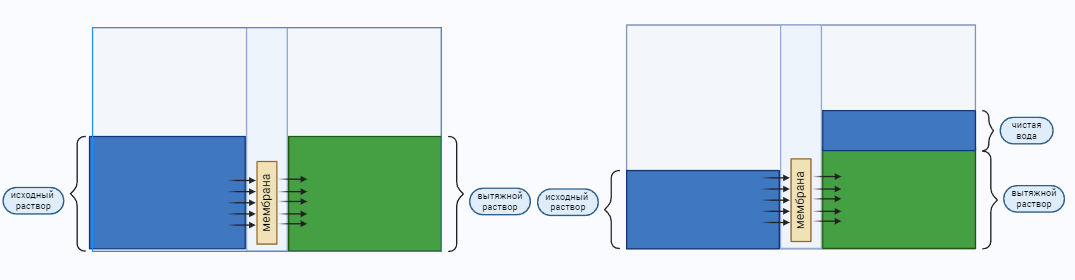
\includegraphics[width=0.8\textwidth]{media/chem/image26}
	\caption*{}
\end{figure}


{\bfseries Рис. 1 -- Визуализированная схема системы прямого осмоса}

\emph{Опреснение морской воды методом прямого осмоса с использованием
растворов хлорида натрия (NaCl)}

В ходе эксперимента в качестве полупроницаемой мембраны применялась
коммерческая мембрана на основе полиакриламидного тонкопленчатого
композита марки Atoll TW40-1812-50 (Тайвань). Коэффициент проницаемости
(L) данной мембраны составляет -- 7,5 л·м⁻²·ч⁻¹/Па а площадь поверхности
мембраны (А) исходя из размера используемой в экспериментальной системе
прямого осмоса полупроницаемой мембраны составляет -- 0,01
м\textsuperscript{2}. А также для постановки эксперимента по опреснению
морской воды были выбраны исходный и вытяжные растворы следующих
составов: в качестве исходного раствора использовалась морская вода (из
Средиземного моря) с содержанием хлорида натрия (NaCl) в массовой
концентрации 3,7\%. Для вытяжных растворов были подготовлены растворы
NaCl с концентрациями 9\%, 18\% и 25\%. Исходные и вытяжные растворы
были взяты для экспериментов по 1000 см³. Пробы для анализа отбирались
каждые 12 часов. Эксперименты проводились при комнатной температуре в
диапазоне 25-28\textsuperscript{0}С. В таблицах 1-3 указаны данные по
проведенному эксперименту по опреснению воды методом прямого осмоса с
использованием раствора хлорида натрия в разных концентрациях в качестве
вытяжного раствора с относительно высоким осмотическим давлением.

{\bfseries Таблица 1 - Опреснение морской воды с использованием 9\% NaCl}

% \begin{longtable}[]{@{}
%   >{\raggedright\arraybackslash}p{(\columnwidth - 18\tabcolsep) * \real{0.0598}}
%   >{\raggedright\arraybackslash}p{(\columnwidth - 18\tabcolsep) * \real{0.0709}}
%   >{\raggedright\arraybackslash}p{(\columnwidth - 18\tabcolsep) * \real{0.0721}}
%   >{\raggedright\arraybackslash}p{(\columnwidth - 18\tabcolsep) * \real{0.0911}}
%   >{\raggedright\arraybackslash}p{(\columnwidth - 18\tabcolsep) * \real{0.1620}}
%   >{\raggedright\arraybackslash}p{(\columnwidth - 18\tabcolsep) * \real{0.0735}}
%   >{\raggedright\arraybackslash}p{(\columnwidth - 18\tabcolsep) * \real{0.0884}}
%   >{\raggedright\arraybackslash}p{(\columnwidth - 18\tabcolsep) * \real{0.1619}}
%   >{\raggedright\arraybackslash}p{(\columnwidth - 18\tabcolsep) * \real{0.1325}}
%   >{\raggedright\arraybackslash}p{(\columnwidth - 18\tabcolsep) * \real{0.0877}}@{}}
% \toprule\noalign{}
% \multicolumn{2}{@{}>{\raggedright\arraybackslash}p{(\columnwidth - 18\tabcolsep) * \real{0.1308} + 2\tabcolsep}}{%
% \multirow{2}{=}{\begin{minipage}[b]{\linewidth}\raggedright
% Время
% \end{minipage}}} &
% \multicolumn{3}{>{\raggedright\arraybackslash}p{(\columnwidth - 18\tabcolsep) * \real{0.3252} + 4\tabcolsep}}{%
% \begin{minipage}[b]{\linewidth}\raggedright
% Начальная концентрация исходного раствора -- 3,7\%
% \end{minipage}} &
% \multicolumn{3}{>{\raggedright\arraybackslash}p{(\columnwidth - 18\tabcolsep) * \real{0.3238} + 4\tabcolsep}}{%
% \begin{minipage}[b]{\linewidth}\raggedright
% Начальная концентрация вытяжного раствора -- 9\%
% \end{minipage}} &
% \multirow{3}{=}{\begin{minipage}[b]{\linewidth}\raggedright
% Δπ, Па
% \end{minipage}} &
% \multirow{3}{=}{\begin{minipage}[b]{\linewidth}\raggedright
% Поток воды J\textsubscript{w},
% 
% л·м⁻²·ч⁻¹
% \end{minipage}} \\
% & &
% \multicolumn{2}{>{\raggedright\arraybackslash}p{(\columnwidth - 18\tabcolsep) * \real{0.1632} + 2\tabcolsep}}{%
% \begin{minipage}[b]{\linewidth}\raggedright
% Концентрация исходного раствора
% \end{minipage}} &
% \multirow{2}{=}{\begin{minipage}[b]{\linewidth}\raggedright
% Осмотическое давление (π) FS, Па
% \end{minipage}} &
% \multicolumn{2}{>{\raggedright\arraybackslash}p{(\columnwidth - 18\tabcolsep) * \real{0.1619} + 2\tabcolsep}}{%
% \begin{minipage}[b]{\linewidth}\raggedright
% Концентрация вытяжного раствора
% \end{minipage}} &
% \multirow{2}{=}{\begin{minipage}[b]{\linewidth}\raggedright
% Осмотическое давление (π) DS, Па
% \end{minipage}} \\
% \begin{minipage}[b]{\linewidth}\raggedright
% час
% \end{minipage} & \begin{minipage}[b]{\linewidth}\raggedright
% день
% \end{minipage} & \begin{minipage}[b]{\linewidth}\raggedright
% \%
% \end{minipage} & \begin{minipage}[b]{\linewidth}\raggedright
% моль/л
% \end{minipage} & & \begin{minipage}[b]{\linewidth}\raggedright
% \%
% \end{minipage} & \begin{minipage}[b]{\linewidth}\raggedright
% моль/л
% \end{minipage} \\
% \midrule\noalign{}
% \endhead
% \bottomrule\noalign{}
% \endlastfoot
% 0 & 0 & 3,7 & 0,632 & -- & 9 & 1,538 & -- & -- & -- \\
% 12 & 0,5 & 3,95 & 0,675 & 1,673*10\textsuperscript{3} & 8,74 & 1,494 &
% 3,702*10\textsuperscript{3} & 2,029*10\textsuperscript{3} & 20,29 \\
% 24 & 1,0 & 4,21 & 0,720 & 1,783*10\textsuperscript{3} & 8,47 & 1,448 &
% 3,587*10\textsuperscript{3} & 1,804*10\textsuperscript{3} & 18,04 \\
% 36 & 1,5 & 4,35 & 0,744 & 1,842*10\textsuperscript{3} & 8,25 & 1,410 &
% 3,494*10\textsuperscript{3} & 1,652*10\textsuperscript{3} & 16,52 \\
% 48 & 2,0 & 4,6 & 0,786 & 1,948*10\textsuperscript{3} & 8,1 & 1,385 &
% 3,430*10\textsuperscript{3} & 1,482*10\textsuperscript{3} & 14,82 \\
% 60 & 2,5 & 4,86 & 0,831 & 2,058*10\textsuperscript{3} & 7,95 & 1,359 &
% 3,367*10\textsuperscript{3} & 1,309*10\textsuperscript{3} & 13,09 \\
% 72 & 3,0 & 4,97 & 0,850 & 2,105*10\textsuperscript{3} & 7,83 & 1,338 &
% 3,316*10\textsuperscript{3} & 1,211*10\textsuperscript{3} & 12,11 \\
% 84 & 3,5 & 5,08 & 0,868 & 2,151*10\textsuperscript{3} & 7,72 & 1,320 &
% 3,270*10\textsuperscript{3} & 1,118*10\textsuperscript{3} & 11,18 \\
% 96 & 4,0 & 5,2 & 0,889 & 2,202*10\textsuperscript{3} & 7,59 & 1,297 &
% 3,214*10\textsuperscript{3} & 1,012*10\textsuperscript{3} & 10,12 \\
% 108 & 4,5 & 5,29 & 0,904 & 2,240*10\textsuperscript{3} & 7,46 & 1,275 &
% 3,159*10\textsuperscript{3} & 0,919*10\textsuperscript{3} & 9,19 \\
% 120 & 5,0 & 5,41 & 0,925 & 2,291*10\textsuperscript{3} & 7,38 & 1,262 &
% 3,126*10\textsuperscript{3} & 0,834*10\textsuperscript{3} & 8,34 \\
% 132 & 5,5 & 5,49 & 0,938 & 2,325*10\textsuperscript{3} & 7,25 & 1,239 &
% 3,070*10\textsuperscript{3} & 0,745*10\textsuperscript{3} & 7,45 \\
% 144 & 6,0 & 5,56 & 0,950 & 2,355*10\textsuperscript{3} & 7,18 & 1,227 &
% 3,041*10\textsuperscript{3} & 0,686*10\textsuperscript{3} & 6,86 \\
% 156 & 6,5 & 5,59 & 0,956 & 2,367*10\textsuperscript{3} & 7,12 & 1,217 &
% 3,015*10\textsuperscript{3} & 0,648*10\textsuperscript{3} & 6,48 \\
% 168 & 7,0 & 5,62 & 0,961 & 2,380*10\textsuperscript{3} & 7,07 & 1,209 &
% 2,994*10\textsuperscript{3} & 0,614*10\textsuperscript{3} & 6,14 \\
% \end{longtable}

{\bfseries Таблица 2 - Опреснение морской воды с использованием 18\% NaCl}

% \begin{longtable}[]{@{}
%   >{\raggedright\arraybackslash}p{(\columnwidth - 18\tabcolsep) * \real{0.0598}}
%   >{\raggedright\arraybackslash}p{(\columnwidth - 18\tabcolsep) * \real{0.0709}}
%   >{\raggedright\arraybackslash}p{(\columnwidth - 18\tabcolsep) * \real{0.0721}}
%   >{\raggedright\arraybackslash}p{(\columnwidth - 18\tabcolsep) * \real{0.1058}}
%   >{\raggedright\arraybackslash}p{(\columnwidth - 18\tabcolsep) * \real{0.1473}}
%   >{\raggedright\arraybackslash}p{(\columnwidth - 18\tabcolsep) * \real{0.0883}}
%   >{\raggedright\arraybackslash}p{(\columnwidth - 18\tabcolsep) * \real{0.0884}}
%   >{\raggedright\arraybackslash}p{(\columnwidth - 18\tabcolsep) * \real{0.1472}}
%   >{\raggedright\arraybackslash}p{(\columnwidth - 18\tabcolsep) * \real{0.1325}}
%   >{\raggedright\arraybackslash}p{(\columnwidth - 18\tabcolsep) * \real{0.0877}}@{}}
% \toprule\noalign{}
% \multicolumn{2}{@{}>{\raggedright\arraybackslash}p{(\columnwidth - 18\tabcolsep) * \real{0.1308} + 2\tabcolsep}}{%
% \multirow{2}{=}{\begin{minipage}[b]{\linewidth}\raggedright
% Время
% \end{minipage}}} &
% \multicolumn{3}{>{\raggedright\arraybackslash}p{(\columnwidth - 18\tabcolsep) * \real{0.3252} + 4\tabcolsep}}{%
% \begin{minipage}[b]{\linewidth}\raggedright
% Начальная концентрация исходного раствора -- 3,7\%
% \end{minipage}} &
% \multicolumn{3}{>{\raggedright\arraybackslash}p{(\columnwidth - 18\tabcolsep) * \real{0.3238} + 4\tabcolsep}}{%
% \begin{minipage}[b]{\linewidth}\raggedright
% Начальная концентрация вытяжного раствора -- 18\%
% \end{minipage}} &
% \multirow{3}{=}{\begin{minipage}[b]{\linewidth}\raggedright
% Δπ, Па
% \end{minipage}} &
% \multirow{3}{=}{\begin{minipage}[b]{\linewidth}\raggedright
% Поток воды J\textsubscript{w}, л·м⁻²·ч⁻¹
% \end{minipage}} \\
% & &
% \multicolumn{2}{>{\raggedright\arraybackslash}p{(\columnwidth - 18\tabcolsep) * \real{0.1779} + 2\tabcolsep}}{%
% \begin{minipage}[b]{\linewidth}\raggedright
% Концентрация исходного раствора
% \end{minipage}} &
% \multirow{2}{=}{\begin{minipage}[b]{\linewidth}\raggedright
% Осмотичес-кое давление (π) FS, Па
% \end{minipage}} &
% \multicolumn{2}{>{\raggedright\arraybackslash}p{(\columnwidth - 18\tabcolsep) * \real{0.1767} + 2\tabcolsep}}{%
% \begin{minipage}[b]{\linewidth}\raggedright
% Концентрация вытяжного раствора
% \end{minipage}} &
% \multirow{2}{=}{\begin{minipage}[b]{\linewidth}\raggedright
% Осмотичес-кое давление (π) DS, Па
% \end{minipage}} \\
% \begin{minipage}[b]{\linewidth}\raggedright
% час
% \end{minipage} & \begin{minipage}[b]{\linewidth}\raggedright
% день
% \end{minipage} & \begin{minipage}[b]{\linewidth}\raggedright
% \%
% \end{minipage} & \begin{minipage}[b]{\linewidth}\raggedright
% моль/л
% \end{minipage} & & \begin{minipage}[b]{\linewidth}\raggedright
% \%
% \end{minipage} & \begin{minipage}[b]{\linewidth}\raggedright
% моль/л
% \end{minipage} \\
% \midrule\noalign{}
% \endhead
% \bottomrule\noalign{}
% \endlastfoot
% 0 & 0 & 3,7 & 0,632 & -- & 18 & 3,077 & -- & -- & -- \\
% 12 & 0,5 & 4,27 & 0,730 & 1,808*10\textsuperscript{3} & 17,43 & 2,979 &
% 7,382*10\textsuperscript{3} & 5,573*10\textsuperscript{3} & 55,7 \\
% 24 & 1,0 & 4,83 & 0,826 & 2,046*10\textsuperscript{3} & 16,87 & 2,884 &
% 7,145*10\textsuperscript{3} & 5,099*10\textsuperscript{3} & 51,0 \\
% 36 & 1,5 & 5,38 & 0,920 & 2,279*10\textsuperscript{3} & 16,32 & 2,790 &
% 6,912*10\textsuperscript{3} & 4,633*10\textsuperscript{3} & 46,3 \\
% 48 & 2,0 & 5,92 & 1,012 & 2,507*10\textsuperscript{3} & 15,78 & 2,697 &
% 6,683*10\textsuperscript{3} & 4,176*10\textsuperscript{3} & 41,8 \\
% 60 & 2,5 & 6,45 & 1,103 & 2,732*10\textsuperscript{3} & 15,25 & 2,607 &
% 6,459*10\textsuperscript{3} & 3,727*10\textsuperscript{3} & 37,3 \\
% 72 & 3,0 & 6,97 & 1,191 & 2,952*10\textsuperscript{3} & 14,73 & 2,518 &
% 6,238*10\textsuperscript{3} & 3,286*10\textsuperscript{3} & 32,9 \\
% 84 & 3,5 & 7,48 & 1,279 & 3,168*10\textsuperscript{3} & 14,22 & 2,431 &
% 6,022*10\textsuperscript{3} & 2,855*10\textsuperscript{3} & 28,5 \\
% 96 & 4,0 & 7,98 & 1,364 & 3,380*10\textsuperscript{3} & 13,72 & 2,345 &
% 5,811*10\textsuperscript{3} & 2,431*10\textsuperscript{3} & 24,3 \\
% 108 & 4,5 & 8,47 & 1,448 & 3,587*10\textsuperscript{3} & 13,23 & 2,262 &
% 5,603*10\textsuperscript{3} & 2,016*10\textsuperscript{3} & 20,2 \\
% 120 & 5,0 & 8,95 & 1,530 & 3,790*10\textsuperscript{3} & 12,75 & 2,179 &
% 5,400*10\textsuperscript{3} & 1,609*10\textsuperscript{3} & 16,1 \\
% 132 & 5,5 & 9,42 & 1,610 & 3,990*10\textsuperscript{3} & 12,28 & 2,099 &
% 5,201*10\textsuperscript{3} & 1,211*10\textsuperscript{3} & 12,1 \\
% 144 & 6,0 & 9,88 & 1,689 & 4,184*10\textsuperscript{3} & 11,82 & 2,021 &
% 5,006*10\textsuperscript{3} & 0,822*10\textsuperscript{3} & 8,2 \\
% 156 & 6,5 & 10,33 & 1,766 & 4,375*10\textsuperscript{3} & 11,37 & 1,944
% & 4,815*10\textsuperscript{3} & 0,440*10\textsuperscript{3} & 4,4 \\
% 168 & 7,0 & 10,77 & 1,841 & 4,561*10\textsuperscript{3} & 10,93 & 1,868
% & 4,629*10\textsuperscript{3} & 0,068*10\textsuperscript{3} & 0,7 \\
% \end{longtable}

{\bfseries Таблица 3 - Опреснение морской воды с использованием 25\% NaCl}

% \begin{longtable}[]{@{}
%   >{\raggedright\arraybackslash}p{(\columnwidth - 18\tabcolsep) * \real{0.0598}}
%   >{\raggedright\arraybackslash}p{(\columnwidth - 18\tabcolsep) * \real{0.0709}}
%   >{\raggedright\arraybackslash}p{(\columnwidth - 18\tabcolsep) * \real{0.0896}}
%   >{\raggedright\arraybackslash}p{(\columnwidth - 18\tabcolsep) * \real{0.0883}}
%   >{\raggedright\arraybackslash}p{(\columnwidth - 18\tabcolsep) * \real{0.1473}}
%   >{\raggedright\arraybackslash}p{(\columnwidth - 18\tabcolsep) * \real{0.0883}}
%   >{\raggedright\arraybackslash}p{(\columnwidth - 18\tabcolsep) * \real{0.0884}}
%   >{\raggedright\arraybackslash}p{(\columnwidth - 18\tabcolsep) * \real{0.1472}}
%   >{\raggedright\arraybackslash}p{(\columnwidth - 18\tabcolsep) * \real{0.1325}}
%   >{\raggedright\arraybackslash}p{(\columnwidth - 18\tabcolsep) * \real{0.0877}}@{}}
% \toprule\noalign{}
% \multicolumn{2}{@{}>{\raggedright\arraybackslash}p{(\columnwidth - 18\tabcolsep) * \real{0.1308} + 2\tabcolsep}}{%
% \multirow{2}{=}{\begin{minipage}[b]{\linewidth}\raggedright
% Время
% \end{minipage}}} &
% \multicolumn{3}{>{\raggedright\arraybackslash}p{(\columnwidth - 18\tabcolsep) * \real{0.3252} + 4\tabcolsep}}{%
% \begin{minipage}[b]{\linewidth}\raggedright
% Начальная концентрация исходного раствора -- 3,7\%
% \end{minipage}} &
% \multicolumn{3}{>{\raggedright\arraybackslash}p{(\columnwidth - 18\tabcolsep) * \real{0.3238} + 4\tabcolsep}}{%
% \begin{minipage}[b]{\linewidth}\raggedright
% Начальная концентрация вытяжного раствора -- 25\%
% \end{minipage}} &
% \multirow{3}{=}{\begin{minipage}[b]{\linewidth}\raggedright
% Δπ, Па
% \end{minipage}} &
% \multirow{3}{=}{\begin{minipage}[b]{\linewidth}\raggedright
% Поток воды J\textsubscript{w}, л·м⁻²·ч⁻¹
% \end{minipage}} \\
% & &
% \multicolumn{2}{>{\raggedright\arraybackslash}p{(\columnwidth - 18\tabcolsep) * \real{0.1779} + 2\tabcolsep}}{%
% \begin{minipage}[b]{\linewidth}\raggedright
% Концентрация исходного раствора
% \end{minipage}} &
% \multirow{2}{=}{\begin{minipage}[b]{\linewidth}\raggedright
% Осмотичес-кое давление (π) FS, Па
% \end{minipage}} &
% \multicolumn{2}{>{\raggedright\arraybackslash}p{(\columnwidth - 18\tabcolsep) * \real{0.1767} + 2\tabcolsep}}{%
% \begin{minipage}[b]{\linewidth}\raggedright
% Концентрация вытяжного раствора
% \end{minipage}} &
% \multirow{2}{=}{\begin{minipage}[b]{\linewidth}\raggedright
% Осмотичес-кое давление (π) DS, Па
% \end{minipage}} \\
% \begin{minipage}[b]{\linewidth}\raggedright
% час
% \end{minipage} & \begin{minipage}[b]{\linewidth}\raggedright
% день
% \end{minipage} & \begin{minipage}[b]{\linewidth}\raggedright
% \%
% \end{minipage} & \begin{minipage}[b]{\linewidth}\raggedright
% моль/л
% \end{minipage} & & \begin{minipage}[b]{\linewidth}\raggedright
% \%
% \end{minipage} & \begin{minipage}[b]{\linewidth}\raggedright
% моль/л
% \end{minipage} \\
% \midrule\noalign{}
% \endhead
% \bottomrule\noalign{}
% \endlastfoot
% 0 & 0 & 3,7 & 0,632 & -- & 25 & 4,274 & -- & -- & -- \\
% 12 & 0,5 & 4,65 & 0,795 & 1,969*10\textsuperscript{3} & 24,04 & 4,109 &
% 1,0181*10\textsuperscript{4} & 8,212*10\textsuperscript{3} & 82,12 \\
% 24 & 1,0 & 5,57 & 0,952 & 2,359*10\textsuperscript{3} & 23,15 & 3,957 &
% 9,804*10\textsuperscript{3} & 7,445*10\textsuperscript{3} & 74,45 \\
% 36 & 1,5 & 6,44 & 1,101 & 2,727*10\textsuperscript{3} & 22,23 & 3,800 &
% 9,415*10\textsuperscript{3} & 6,687*10\textsuperscript{3} & 66,87 \\
% 48 & 2,0 & 7,25 & 1,239 & 3,070*10\textsuperscript{3} & 21,46 & 3,668 &
% 9,089*10\textsuperscript{3} & 6,018*10\textsuperscript{3} & 60,18 \\
% 60 & 2,5 & 8,01 & 1,369 & 3,392*10\textsuperscript{3} & 20,68 & 3,535 &
% 8,758*10\textsuperscript{3} & 5,366*10\textsuperscript{3} & 53,66 \\
% 72 & 3,0 & 8,72 & 1,491 & 3,693*10\textsuperscript{3} & 19,95 & 3,410 &
% 8,449*10\textsuperscript{3} & 4,756*10\textsuperscript{3} & 47,56 \\
% 84 & 3,5 & 9,38 & 1,603 & 3,973*10\textsuperscript{3} & 19,31 & 3,301 &
% 8,178*10\textsuperscript{3} & 4,206*10\textsuperscript{3} & 42,06 \\
% 96 & 4,0 & 10 & 1,709 & 4,235*10\textsuperscript{3} & 18,72 & 3,200 &
% 7,928*10\textsuperscript{3} & 3,693*10\textsuperscript{3} & 36,93 \\
% 108 & 4,5 & 10,58 & 1,809 & 4,481*10\textsuperscript{3} & 18,13 & 3,099
% & 7,678*10\textsuperscript{3} & 3,198*10\textsuperscript{3} & 31,98 \\
% 120 & 5,0 & 11,11 & 1,899 & 4,705*10\textsuperscript{3} & 17,57 & 3,003
% & 7,441*10\textsuperscript{3} & 2,736*10\textsuperscript{3} & 27,36 \\
% 132 & 5,5 & 11,61 & 1,985 & 4,917*10\textsuperscript{3} & 17,05 & 2,915
% & 7,221*10\textsuperscript{3} & 2,304*10\textsuperscript{3} & 23,04 \\
% 144 & 6,0 & 12,07 & 2,063 & 5,112*10\textsuperscript{3} & 16,65 & 2,846
% & 7,052*10\textsuperscript{3} & 1,940*10\textsuperscript{3} & 19,40 \\
% 156 & 6,5 & 12,48 & 2,133 & 5,285*10\textsuperscript{3} & 16,2 & 2,769 &
% 6,861*10\textsuperscript{3} & 1,575*10\textsuperscript{3} & 15,75 \\
% 168 & 7,0 & 12,86 & 2,198 & 5,446*10\textsuperscript{3} & 15,83 & 2,706
% & 6,704*10\textsuperscript{3} & 1,258*10\textsuperscript{3} & 12,58 \\
% 180 & 7,5 & 13,2 & 2,256 & 5,590*10\textsuperscript{3} & 15,54 & 2,656 &
% 6,581*10\textsuperscript{3} & 0,991*10\textsuperscript{3} & 9,91 \\
% 192 & 8,0 & 13,51 & 2,309 & 5,722*10\textsuperscript{3} & 15,21 & 2,600
% & 6,442*10\textsuperscript{3} & 0,720*10\textsuperscript{3} & 7,20 \\
% 204 & 8,5 & 13,76 & 2,352 & 5,828*10\textsuperscript{3} & 14,92 & 2,550
% & 6,319*10\textsuperscript{3} & 0,491*10\textsuperscript{3} & 4,91 \\
% 216 & 9,0 & 13,97 & 2,388 & 5,917*10\textsuperscript{3} & 14,75 & 2,521
% & 6,247*10\textsuperscript{3} & 0,330*10\textsuperscript{3} & 3,30 \\
% 228 & 9,5 & 14,13 & 2,415 & 5,984*10\textsuperscript{3} & 14,57 & 2,491
% & 6,171*10\textsuperscript{3} & 0,186*10\textsuperscript{3} & 1,86 \\
% 240 & 10,0 & 14,24 & 2,434 & 6,031*10\textsuperscript{3} & 14,45 & 2,470
% & 6,120*10\textsuperscript{3} & 0,089*10\textsuperscript{3} & 0,89 \\
% 252 & 10.5 & 14,31 & 2,446 & 6,061*10\textsuperscript{3} & 14,36 & 2,455
% & 6,082*10\textsuperscript{3} & 0,021*10\textsuperscript{3} & - \\
% \end{longtable}

Из полученных данных экспериментов по опреснению соленой морской воды
методом прямого осмоса с применением полупроницаемой мембраны и с
использованием в качестве вытяжного раствора хлорида натрия в различных
концентрациях для большей достоверность эксперимента можем наблюдать
прямую зависимость между концентрацией и осмотическим давлением
вытяжного раствора потоком воды через полупроницаемую мембрану. С
увеличением концентрации вытяжного раствора в виде хлорида натрия в
порядке 9\%, 18\% и 25\% поток воды увеличивается в соответствующем
порядке -- 20,29 л·м⁻²·ч⁻¹, 55,7 л·м⁻²·ч⁻¹ и 81,12 л·м⁻²·ч⁻¹. Также, по
данным, указанным в таблицах 1-3, можно сделать вывод, что с увеличением
концентрации исходного раствора поток воды уменьшается в линейной
завистимости. Это доказывает уменьшение скорости притока чистой воды в
отсек с вытяжным раствором. Высокая концентрация вытяжного раствора
приводит к повышению осмотического давления, что стимулирует большой
поток воды через мембрану. Это указывает на эффективность процесса
прямого осмоса при использовании более концентрированных вытяжных
растворов. Анализируя вышеуказанные данные в таблицах 1-3, можем
заметить, что, в связи с выравниванием концентрации исходного и
вытяжного растворов поток воды уменьшается. Исследована зависимость
потока воды от времени, результаты которого приведены на рисунке 3.

\begin{figure}[H]
	\centering
	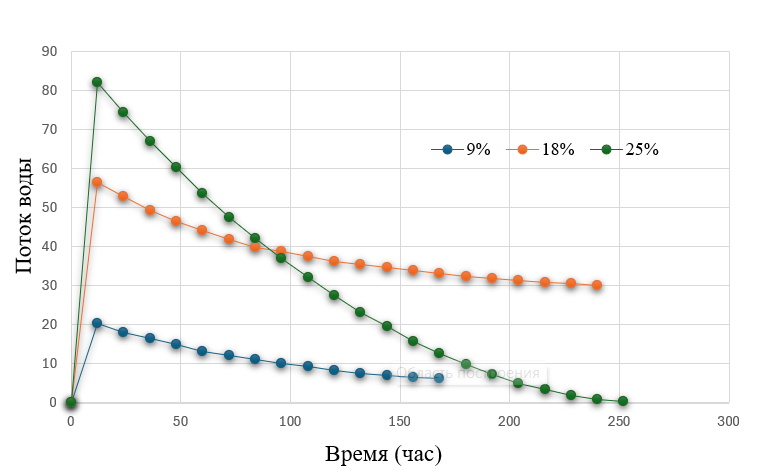
\includegraphics[width=0.8\textwidth]{media/chem/image27}
	\caption*{}
\end{figure}


{\bfseries Рис. 3 - Влияние концентрации вытяжного раствора на поток воды в
зависимости от времени в процессе прямого осмоса}

В процессе опреснения морской воды методом прямого осмоса
концентрированный раствор разбавляется за счет потока молекул воды через
полупроницаемую мембрану до выравнивания осмотического давления.
Регенерация чистой воды из разбавленного вытяжного раствора проводится
путем дистилляции раствора. При опреснении методом прямого осмоса с
использованием растворов хлорида натрия в различных концентрациях были
получены следующие результаты. При концентрации NaCl 9\% объем чистой
пресной воды составил 272 см³. При увеличении концентрации NaCl до 18\%
объем чистой воды увеличился до 647 см³. Наибольший объем чистой воды,
равный 741 см³, был получен при концентрации раствора хлорида натрия
25\%. Таким образом, можно сделать вывод, что с увеличением массовой
концентрации раствора хлорида натрия используемый в качестве вытяжного
раствора объем получаемой чистой воды также увеличивается.

Процесс прямого осмоса является неотъемлемой частью зеленой химии, так
как он позволяет обеспечить доступ к пресной воде без использования
дорогостоящих химических реагентов или энергозатратных высоких
температур, что снижает воздействие на окружающую среду и природные
ресурсы.

Увеличение максимального потока воды при повышении концентрации
вытяжного раствора свидетельствует о быстром и эффективном процессе
опреснения соленой морской воды, что может быть важным фактором в
обеспечении доступа к пресной воде в регионах с ограниченными ресурсами.

Таким образом, результаты эксперимента демонстрируют значительный
потенциал прямого осмоса с применением концентрированных растворов
хлорида натрия в качестве вытяжных растворов для эффективного,
недорогого и быстрого опреснения соленых вод, что важно для решения
проблем доступа к чистой воде в масштабах планеты.

\emph{Опреснение морской воды из Каспийского моря методом прямого
осмоса}

Данный эксперимент по опреснению морской соленой воды проводился
аналогично вышеуказанному эксперименту. Для постановки эксперимента по
опреснению морской воды были выбраны исходный и вытяжной растворы
следующих составов: в качестве исходного раствора использовалась морская
вода (из Каспийского моря) с содержанием хлорида натрия (NaCl) в
концентрации 1.6 \%. Для вытяжного раствора был подготовлен раствор NaCl
с концентрацией 25\%, так как, проведенный ранее эксперимент указывает
что, для достижения максимального потока воды в процессе опреснения воды
методом прямого осмоса в качестве вытяжного раствора эффективно
использовать растворов с высокой концентрацией. Пробы для анализа
отбирались каждые 12 часов в течение 7 календарных дней. Эксперименты
проводились при комнатной температуре 25°С. В таблице 4 указаны данные
по проведенному эксперименту по опреснению воды методом прямого осмоса с
использованием раствора хлорида натрия в концентрации 25\% в качестве
вытяжного раствора с относительно высоким осмотическим давлением.

{\bfseries Таблица 4 - Опреснение морской воды из Каспийского моря с
использованием 25\% NaCl}

% \begin{longtable}[]{@{}
%   >{\raggedright\arraybackslash}p{(\columnwidth - 18\tabcolsep) * \real{0.0598}}
%   >{\raggedright\arraybackslash}p{(\columnwidth - 18\tabcolsep) * \real{0.0709}}
%   >{\raggedright\arraybackslash}p{(\columnwidth - 18\tabcolsep) * \real{0.0896}}
%   >{\raggedright\arraybackslash}p{(\columnwidth - 18\tabcolsep) * \real{0.0882}}
%   >{\raggedright\arraybackslash}p{(\columnwidth - 18\tabcolsep) * \real{0.1618}}
%   >{\raggedright\arraybackslash}p{(\columnwidth - 18\tabcolsep) * \real{0.0736}}
%   >{\raggedright\arraybackslash}p{(\columnwidth - 18\tabcolsep) * \real{0.0883}}
%   >{\raggedright\arraybackslash}p{(\columnwidth - 18\tabcolsep) * \real{0.1618}}
%   >{\raggedright\arraybackslash}p{(\columnwidth - 18\tabcolsep) * \real{0.1177}}
%   >{\raggedright\arraybackslash}p{(\columnwidth - 18\tabcolsep) * \real{0.0882}}@{}}
% \toprule\noalign{}
% \multicolumn{2}{@{}>{\raggedright\arraybackslash}p{(\columnwidth - 18\tabcolsep) * \real{0.1307} + 2\tabcolsep}}{%
% \multirow{2}{=}{\begin{minipage}[b]{\linewidth}\raggedright
% Время
% \end{minipage}}} &
% \multicolumn{3}{>{\raggedright\arraybackslash}p{(\columnwidth - 18\tabcolsep) * \real{0.3396} + 4\tabcolsep}}{%
% \begin{minipage}[b]{\linewidth}\raggedright
% Начальная концентрация исходного раствора -- 3,7\%
% \end{minipage}} &
% \multicolumn{3}{>{\raggedright\arraybackslash}p{(\columnwidth - 18\tabcolsep) * \real{0.3237} + 4\tabcolsep}}{%
% \begin{minipage}[b]{\linewidth}\raggedright
% Начальная концентрация вытяжного раствора -- 25\%
% \end{minipage}} &
% \multirow{3}{=}{\begin{minipage}[b]{\linewidth}\raggedright
% Δπ, Па
% \end{minipage}} &
% \multirow{3}{=}{\begin{minipage}[b]{\linewidth}\raggedright
% Поток воды J\textsubscript{w}, л·м⁻²·ч⁻¹
% \end{minipage}} \\
% & &
% \multicolumn{2}{>{\raggedright\arraybackslash}p{(\columnwidth - 18\tabcolsep) * \real{0.1778} + 2\tabcolsep}}{%
% \begin{minipage}[b]{\linewidth}\raggedright
% Концентрация исходного раствора
% \end{minipage}} &
% \multirow{2}{=}{\begin{minipage}[b]{\linewidth}\raggedright
% Осмотическое давление (π) FS, Па
% \end{minipage}} &
% \multicolumn{2}{>{\raggedright\arraybackslash}p{(\columnwidth - 18\tabcolsep) * \real{0.1619} + 2\tabcolsep}}{%
% \begin{minipage}[b]{\linewidth}\raggedright
% Концентрация вытяжного раствора
% \end{minipage}} &
% \multirow{2}{=}{\begin{minipage}[b]{\linewidth}\raggedright
% Осмотическое- давление (π) DS, Па
% \end{minipage}} \\
% \begin{minipage}[b]{\linewidth}\raggedright
% час
% \end{minipage} & \begin{minipage}[b]{\linewidth}\raggedright
% день
% \end{minipage} & \begin{minipage}[b]{\linewidth}\raggedright
% \%
% \end{minipage} & \begin{minipage}[b]{\linewidth}\raggedright
% моль/л
% \end{minipage} & & \begin{minipage}[b]{\linewidth}\raggedright
% \%
% \end{minipage} & \begin{minipage}[b]{\linewidth}\raggedright
% моль/л
% \end{minipage} \\
% \midrule\noalign{}
% \endhead
% \bottomrule\noalign{}
% \endlastfoot
% 0 & 0 & 1,6 & 0,274 & -- & 25 & 4,274 & -- & -- & -- \\
% 12 & 0,5 & 2,55 & 0,436 & 1,080*10\textsuperscript{3} & 24,04 & 4,109 &
% 1,018*10\textsuperscript{4} & 9,100*10\textsuperscript{3} & 91,0 \\
% 24 & 1 & 3,47 & 0,593 & 1,470*10\textsuperscript{3} & 23,15 & 3,957 &
% 9,804*10\textsuperscript{3} & 8,334*10\textsuperscript{3} & 83,3 \\
% 36 & 1,5 & 4,34 & 0,742 & 1,838*10\textsuperscript{3} & 22,23 & 3,8 &
% 9,415*10\textsuperscript{3} & 7,577*10\textsuperscript{3} & 75,8 \\
% 48 & 2 & 5,15 & 0,880 & 2,181*10\textsuperscript{3} & 21,46 & 3,668 &
% 9,088*10\textsuperscript{3} & 6,907*10\textsuperscript{3} & 69,1 \\
% 60 & 2,5 & 5,91 & 1,010 & 2,503*10\textsuperscript{3} & 20,68 & 3,535 &
% 8,758*10\textsuperscript{3} & 6,255*10\textsuperscript{3} & 62,6 \\
% 72 & 3 & 6,62 & 1,132 & 2,804*10\textsuperscript{3} & 19,95 & 3,41 &
% 8,449*10\textsuperscript{3} & 5,645*10\textsuperscript{3} & 56,4 \\
% 84 & 3,5 & 7,28 & 1,244 & 3,083*10\textsuperscript{3} & 19,31 & 3,301 &
% 8,178*10\textsuperscript{3} & 5,095*10\textsuperscript{3} & 51,0 \\
% 96 & 4 & 7,9 & 1,350 & 3,346*10\textsuperscript{3} & 18,72 & 3,2 &
% 7,928*10\textsuperscript{3} & 4,582*10\textsuperscript{3} & 45,8 \\
% 108 & 4,5 & 8,48 & 1,450 & 3,591*10\textsuperscript{3} & 18,13 & 3,099 &
% 7,678*10\textsuperscript{3} & 4,087*10\textsuperscript{3} & 40,9 \\
% 120 & 5 & 9,01 & 1,540 & 3,816*10\textsuperscript{3} & 17,57 & 3,003 &
% 7,440*10\textsuperscript{3} & 3,624*10\textsuperscript{3} & 36,2 \\
% 132 & 5,5 & 9,51 & 1,626 & 4,028*10\textsuperscript{3} & 17,05 & 2,915 &
% 7,222*10\textsuperscript{3} & 3,194*10\textsuperscript{3} & 31,9 \\
% 144 & 6 & 9,97 & 1,704 & 4,222*10\textsuperscript{3} & 16,65 & 2,846 &
% 7,051*10\textsuperscript{3} & 2,829*10\textsuperscript{3} & 28,3 \\
% 156 & 6,5 & 10,38 & 1,774 & 4,396*10\textsuperscript{3} & 16,2 & 2,769 &
% 6,860*10\textsuperscript{3} & 2,464*10\textsuperscript{3} & 24,6 \\
% 168 & 7 & 10,76 & 1,839 & 4,557*10\textsuperscript{3} & 15,83 & 2,706 &
% 6,704*10\textsuperscript{3} & 2,147*10\textsuperscript{3} & 21,5 \\
% \end{longtable}

На основе полученных данных по поставленному опыту на протяжении 7
календарных дней по опреснению морской соленой воды методом прямого
осмоса так же наблюдаем тенденцию: чем выше концентрация вытяжного
раствора, тем больше потока воды проходящая через полупроницаемую
мембрану. Соответственно, максимальный поток воды при использовании 25\%
раствора хлорида натрия для опреснения морской воды с содержанием
хлорида натрия -- 1,6\% составила - 91,0 л·м⁻²·ч⁻¹. Нужно заметить,
максимальные потоки воды фиксируются на первых сутках эксперимента. В
том числе высокий поток чистой воды обеспечивает относительно низкая
концентрация солености воды Каспийского моря, которая составляет 1,6\%
чем соленой воды Средиземного моря. Возрастание потока воды при
использовании в качестве исходного раствора морскую воду с более низкой
концентрацией соли объясняется с меньшим загрязнением используемой
мембраны и с низкой степенью отторжения солей. В процессе опреснения
морской воды методом прямого осмоса концентрированный раствор
разбавляется за счет потока молекул воды через полупроницаемую мембрану
до выравнивания осмотического давления. Объем чистой пресной воды
полученной из морской воды Каспийского моря методом прямого осмоса
составил 579 см\textsuperscript{3}. Чистую воду получили методом
термической дистилляции из полученного после процесса опреснения воды
методом прямого осмоса вытяжного раствора (разбавленный чистой водой).
Объем полученной чистой воды был оценен не учитывая объем воды
израсходованная для приготовления вытяжного раствора в виде хлорида
натрия с массовой концентрацией 25\%.

Следовательно, результаты эксперимента подтверждают значительный
потенциал прямого осмоса с использованием концентрированных растворов
хлорида натрия в качестве вытяжных растворов для эффективного,
экономичного и быстрого опреснения соленых вод. Это имеет важное
значение для решения проблемы доступа к чистой воде во всем мире,
включая Казахстан.

\emph{Опреснение морской воды методом прямого осмоса с использованием
растворов сахарозы}

Углеводы, такие как сахароза, фруктоза, глюкоза и другие, благодаря
своему высокому осмотическому давлению, могут успешно применяться в
качестве эффективных вытяжных растворов для процесса опреснения морской
соленой воды методом прямого осмоса, иногда их совместном использовании.
Использование сахарозы, фруктозы и других позволяет производить питьевую
воду, содержащую сахар в качестве водного энергетического напитка как
альтернатива питьевой воды {[}23{]}.

Опреснение морской воды производился с применением 35\% и 70\% растворов
сахарозы в известных массовых концентрациях. Все процедуры по опреснению
морской воды методом прямого осмоса выполнялись в аналогическом порядке
и предыдущим экспериментом. В качестве соленой воды был использован
раствор хлорида натрия с массовой концентрацией 3,5 \%. Концентрация
растворов была определена методом рефрактометрии. Пробы для анализов
отбирались каждые 24 часов. Полученные данные по итогу эксперимента были
изложены в таблицах 5-6.

{\bfseries Таблица 5 - Опреснение соленой воды с использованием 5\%
раствора сахарозы}

% \begin{longtable}[]{@{}
%   >{\raggedright\arraybackslash}p{(\columnwidth - 16\tabcolsep) * \real{0.1026}}
%   >{\raggedright\arraybackslash}p{(\columnwidth - 16\tabcolsep) * \real{0.0882}}
%   >{\raggedright\arraybackslash}p{(\columnwidth - 16\tabcolsep) * \real{0.1177}}
%   >{\raggedright\arraybackslash}p{(\columnwidth - 16\tabcolsep) * \real{0.1472}}
%   >{\raggedright\arraybackslash}p{(\columnwidth - 16\tabcolsep) * \real{0.0882}}
%   >{\raggedright\arraybackslash}p{(\columnwidth - 16\tabcolsep) * \real{0.0883}}
%   >{\raggedright\arraybackslash}p{(\columnwidth - 16\tabcolsep) * \real{0.1471}}
%   >{\raggedright\arraybackslash}p{(\columnwidth - 16\tabcolsep) * \real{0.1324}}
%   >{\raggedright\arraybackslash}p{(\columnwidth - 16\tabcolsep) * \real{0.0882}}@{}}
% \toprule\noalign{}
% \multirow{2}{=}{\begin{minipage}[b]{\linewidth}\raggedright
% Время
% \end{minipage}} &
% \multicolumn{3}{>{\raggedright\arraybackslash}p{(\columnwidth - 16\tabcolsep) * \real{0.3531} + 4\tabcolsep}}{%
% \begin{minipage}[b]{\linewidth}\raggedright
% Начальная концентрация исходного раствора -- 3,5\%
% \end{minipage}} &
% \multicolumn{3}{>{\raggedright\arraybackslash}p{(\columnwidth - 16\tabcolsep) * \real{0.3236} + 4\tabcolsep}}{%
% \begin{minipage}[b]{\linewidth}\raggedright
% Начальная концентрация вытяжного раствора -- 35\%
% \end{minipage}} &
% \multirow{3}{=}{\begin{minipage}[b]{\linewidth}\raggedright
% Δπ, Па
% \end{minipage}} &
% \multirow{3}{=}{\begin{minipage}[b]{\linewidth}\raggedright
% Поток воды J\textsubscript{w}, л·м⁻²·ч⁻¹
% \end{minipage}} \\
% &
% \multicolumn{2}{>{\raggedright\arraybackslash}p{(\columnwidth - 16\tabcolsep) * \real{0.2059} + 2\tabcolsep}}{%
% \begin{minipage}[b]{\linewidth}\raggedright
% Концентрация исходного раствора
% \end{minipage}} &
% \multirow{2}{=}{\begin{minipage}[b]{\linewidth}\raggedright
% Осмотичес-кое давление (π) FS, Па
% \end{minipage}} &
% \multicolumn{2}{>{\raggedright\arraybackslash}p{(\columnwidth - 16\tabcolsep) * \real{0.1766} + 2\tabcolsep}}{%
% \begin{minipage}[b]{\linewidth}\raggedright
% Концентрация вытяжного раствора
% \end{minipage}} &
% \multirow{2}{=}{\begin{minipage}[b]{\linewidth}\raggedright
% Осмотичес-кое давление (π) DS, Па
% \end{minipage}} \\
% \begin{minipage}[b]{\linewidth}\raggedright
% день
% \end{minipage} & \begin{minipage}[b]{\linewidth}\raggedright
% \%
% \end{minipage} & \begin{minipage}[b]{\linewidth}\raggedright
% моль/л
% \end{minipage} & & \begin{minipage}[b]{\linewidth}\raggedright
% \%
% \end{minipage} & \begin{minipage}[b]{\linewidth}\raggedright
% моль/л
% \end{minipage} \\
% \midrule\noalign{}
% \endhead
% \bottomrule\noalign{}
% \endlastfoot
% 0 & 3,5 & 0,598 & -- & 35 & 1,023 & -- & -- & -- \\
% 1 & 3,97 & 0,679 & 1,681*10\textsuperscript{3} & 34,75 & 1,016 &
% 2,517*10\textsuperscript{3} & 0,836*10\textsuperscript{3} & 8,36 \\
% 2 & 4,42 & 0,756 & 1,872*10\textsuperscript{3} & 34,27 & 1,002 &
% 2,483*10\textsuperscript{3} & 0,611*10\textsuperscript{3} & 6,11 \\
% 3 & 4,83 & 0,826 & 2,046*10\textsuperscript{3} & 33,86 & 0,990 &
% 2,453*10\textsuperscript{3} & 0,407*10\textsuperscript{3} & 4,07 \\
% 4 & 5,21 & 0,891 & 2,207*10\textsuperscript{3} & 33,5 & 0,980 &
% 2,427*10\textsuperscript{3} & 0,220*10\textsuperscript{3} & 2,20 \\
% 5 & 5,54 & 0,947 & 2,346*10\textsuperscript{3} & 33,16 & 0,970 &
% 2,402*10\textsuperscript{3} & 0,056*10\textsuperscript{3} & 0,56 \\
% \end{longtable}

{\bfseries Таблица 6 - Опреснение соленой воды с использованием 70\%
раствора сахарозы}

% \begin{longtable}[]{@{}
%   >{\raggedright\arraybackslash}p{(\columnwidth - 16\tabcolsep) * \real{0.1026}}
%   >{\raggedright\arraybackslash}p{(\columnwidth - 16\tabcolsep) * \real{0.0882}}
%   >{\raggedright\arraybackslash}p{(\columnwidth - 16\tabcolsep) * \real{0.1177}}
%   >{\raggedright\arraybackslash}p{(\columnwidth - 16\tabcolsep) * \real{0.1618}}
%   >{\raggedright\arraybackslash}p{(\columnwidth - 16\tabcolsep) * \real{0.0736}}
%   >{\raggedright\arraybackslash}p{(\columnwidth - 16\tabcolsep) * \real{0.0883}}
%   >{\raggedright\arraybackslash}p{(\columnwidth - 16\tabcolsep) * \real{0.1618}}
%   >{\raggedright\arraybackslash}p{(\columnwidth - 16\tabcolsep) * \real{0.1177}}
%   >{\raggedright\arraybackslash}p{(\columnwidth - 16\tabcolsep) * \real{0.0882}}@{}}
% \toprule\noalign{}
% \multirow{2}{=}{\begin{minipage}[b]{\linewidth}\raggedright
% Время
% \end{minipage}} &
% \multicolumn{3}{>{\raggedright\arraybackslash}p{(\columnwidth - 16\tabcolsep) * \real{0.3678} + 4\tabcolsep}}{%
% \begin{minipage}[b]{\linewidth}\raggedright
% Начальная концентрация исходного раствора -- 3,5\%
% \end{minipage}} &
% \multicolumn{3}{>{\raggedright\arraybackslash}p{(\columnwidth - 16\tabcolsep) * \real{0.3237} + 4\tabcolsep}}{%
% \begin{minipage}[b]{\linewidth}\raggedright
% Начальная концентрация вытяжного раствора -- 70\%
% \end{minipage}} &
% \multirow{3}{=}{\begin{minipage}[b]{\linewidth}\raggedright
% Δπ, Па
% \end{minipage}} &
% \multirow{3}{=}{\begin{minipage}[b]{\linewidth}\raggedright
% Поток воды J\textsubscript{w}, л·м⁻²·ч⁻¹
% \end{minipage}} \\
% &
% \multicolumn{2}{>{\raggedright\arraybackslash}p{(\columnwidth - 16\tabcolsep) * \real{0.2059} + 2\tabcolsep}}{%
% \begin{minipage}[b]{\linewidth}\raggedright
% Концентрация исходного раствора
% \end{minipage}} &
% \multirow{2}{=}{\begin{minipage}[b]{\linewidth}\raggedright
% Осмотическое давление (π) FS, Па
% \end{minipage}} &
% \multicolumn{2}{>{\raggedright\arraybackslash}p{(\columnwidth - 16\tabcolsep) * \real{0.1619} + 2\tabcolsep}}{%
% \begin{minipage}[b]{\linewidth}\raggedright
% Концентрация вытяжного раствора
% \end{minipage}} &
% \multirow{2}{=}{\begin{minipage}[b]{\linewidth}\raggedright
% Осмотическое давление (π) DS, Па
% \end{minipage}} \\
% \begin{minipage}[b]{\linewidth}\raggedright
% день
% \end{minipage} & \begin{minipage}[b]{\linewidth}\raggedright
% \%
% \end{minipage} & \begin{minipage}[b]{\linewidth}\raggedright
% моль/л
% \end{minipage} & & \begin{minipage}[b]{\linewidth}\raggedright
% \%
% \end{minipage} & \begin{minipage}[b]{\linewidth}\raggedright
% моль/л
% \end{minipage} \\
% \midrule\noalign{}
% \endhead
% \bottomrule\noalign{}
% \endlastfoot
% 0 & 3,5 & 0,598 & -- & 70 & 2,047 & -- & -- & -- \\
% 1 & 4,45 & 0,761 & 1,885*10\textsuperscript{3} & 69,26 & 2,025 &
% 5,017*10\textsuperscript{3} & 3,133*10\textsuperscript{3} & 31,33 \\
% 2 & 5,37 & 0,918 & 2,274*10\textsuperscript{3} & 68,34 & 1,998 &
% 4,951*10\textsuperscript{3} & 2,677*10\textsuperscript{3} & 26,77 \\
% 3 & 6,24 & 1,067 & 2,643*10\textsuperscript{3} & 67,45 & 1,972 &
% 4,886*10\textsuperscript{3} & 2,244*10\textsuperscript{3} & 22,44 \\
% 4 & 7,05 & 1,205 & 2,986*10\textsuperscript{3} & 66,65 & 1,949 &
% 4,828*10\textsuperscript{3} & 1,843*10\textsuperscript{3} & 18,43 \\
% 5 & 7,81 & 1,335 & 3,308*10\textsuperscript{3} & 65,89 & 1,927 &
% 4,773*10\textsuperscript{3} & 1,466*10\textsuperscript{3} & 14,66 \\
% 6 & 8,52 & 1,456 & 3,608*10\textsuperscript{3} & 65,17 & 1,906 &
% 4,721*10\textsuperscript{3} & 1,113*10\textsuperscript{3} & 11,13 \\
% 7 & 9,18 & 1,569 & 3,888*10\textsuperscript{3} & 64,51 & 1,886 &
% 4,673*10\textsuperscript{3} & 0,785*10\textsuperscript{3} & 7,85 \\
% 8 & 9,8 & 1,675 & 4,150*10\textsuperscript{3} & 63,93 & 1,869 &
% 4,631*10\textsuperscript{3} & 0,481*10\textsuperscript{3} & 4,81 \\
% 9 & 10,38 & 1,774 & 4,396*10\textsuperscript{3} & 63,32 & 1,851 &
% 4,587*10\textsuperscript{3} & 0,191*10\textsuperscript{3} & 1,91 \\
% \end{longtable}

Исходя из полученных данных очередной раз удостоверяемся, что поток воды
при прямом осмосе зависит от концентрации вытяжного раствора. По
полученным данным можем сказать величина потока воды увеличивается с
повышением концентрации вытяжного раствора. Максимальный поток воды
достигается в течение первого дня процесса прямого осмоса при массовой
концентрации вытяжного раствора 70\%. Значение максимального потока --
31,33 л·м⁻²·ч⁻¹. Уменьшение величины потока воды через мембрану
происходит после первого дня. Это говорит о том, что значение потока
чистой воды уменьшается с увеличением времени работы. Чем выше объема
потока вещества, проходящей через полупроницаемую мембрану в процессе
прямого осмоса, тем ниже значения потока воды, образующегося из-за
снижения осмотического давления за счет разбавления раствора. Кроме
того, уменьшение потока чистой воды с увеличением времени связано с
возникновением концентрационной поляризации на поверхности мембраны
{[}24{]}. Влияние концентрации вытяжного раствора на поток воды показано
на рисунке 4.

\begin{figure}[H]
	\centering
	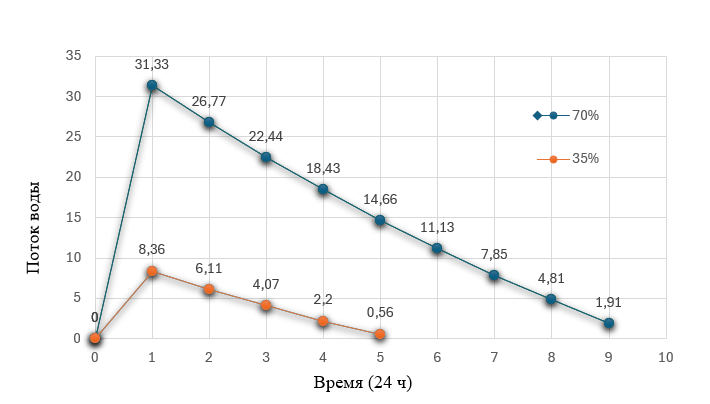
\includegraphics[width=0.8\textwidth]{media/chem/image28}
	\caption*{}
\end{figure}


{\bfseries Рис. 4 -- Влияние концентрации вытяжного раствора на поток воды
в зависимости от времени в процессе прямого осмоса}

Объем полученной чистой воды в двух экспериментах с 35\% и 70\%
сахарозой в качестве вытяжного раствора составил соответственно 54
см\textsuperscript{3} и 105 см\textsuperscript{3}. Один из перспективных
методов опреснения, прямой осмос с использованием растворов сахарозы в
качестве вытяжного раствора, привлекает внимание эффективностью и
потенциалом. Процесс прямого осмоса с применением сахарозы в качестве
вытяжного раствора не требует высоких давлений, что снижает
энергозатраты по сравнению с обратным осмосом. Сахароза является
биоразлагаемым органическим соединение, что делает ее безопасной для
окружающей среды и принимает тенденцию «зеленой химии». Этот метод
обещает эффективное разведение солей и может стать значимым в решении
проблемы доступа к пресной воде. Однако для его широкого применения
необходимы дальнейшие исследования, направленные на оптимизацию условий
процесса и выбор оптимальных мембран, чтобы достичь максимальной
эффективности и экономической целесообразности.

\emph{Опреснение морской воды методом прямого осмоса с использованием
бикарбоната аммония}

Прямой осмос -- это метод, где отделение воды от сырья происходит без
использования внешнего давления. Движущей силой для этого процесса
служит естественный осмотический градиент давления, который возникает
между двумя сторонами полупроницаемой мембраны и способствует диффузии.
Идеальный вытяжной раствор должен обладать повышенным осмотическим
давлением и надежными характеристиками потока воды. Он должен легко
регенерироваться при низких затратах, не содержать токсичных веществ,
иметь возможность повторного использования и обеспечивать минимальный
обратный поток.

Соли аммония действительно обладают рядом подходящих свойств для
использования в качестве вытяжного раствора. При растворении в воде соли
аммония ионизируются, образуя ионы, способные создавать раствор с
высоким осмотическим давлением. Это повышенное осмотическое давление
позволяет увеличить поток воды.

Кроме того, отделение соли аммония на последующем этапе не представляет
сложности. При нагревании при умеренных температурах растворенные соли
аммония, такие как бикарбонат аммония, легко отделяются путем распада на
углекислый газ, газообразный аммиак и воду. Универсальность аммонийных
солей делает их перспективными кандидатами в качестве вытяжного
раствора. Одним из ключевых свойств этого раствора для вытяжки является
его специфическое соотношение аммиака и углекислого газа. При увеличении
концентрации аммиака формируется больше карбоната, что приводит к
повышению осмотического давления вытяжного раствора.

Бикарбонат аммония выделяется из раствора при нагревании в виде
разложившегося аммиака и углекислого газа. Основная реакция этого
явления приведена ниже.

% \begin{longtable}[]{@{}
%   >{\raggedright\arraybackslash}p{(\columnwidth - 2\tabcolsep) * \real{0.9052}}
%   >{\raggedright\arraybackslash}p{(\columnwidth - 2\tabcolsep) * \real{0.0948}}@{}}
% \toprule\noalign{}
% \begin{minipage}[b]{\linewidth}\raggedright
% NH\textsubscript{4}HCO\textsubscript{3}~(водн.)~~↔~~NH\textsubscript{4~}\textsuperscript{+}~(водн.)~~+~~HCO\textsubscript{3}\textsuperscript{−}~(водн.)~~↔
% 
% ↔~NH\textsubscript{3}~(г)~+~CO\textsubscript{2}~(г)~+~H\textsubscript{2}O
% (ж)
% \end{minipage} & \begin{minipage}[b]{\linewidth}\raggedright
% (4)
% \end{minipage} \\
% \midrule\noalign{}
% \endhead
% \bottomrule\noalign{}
% \endlastfoot
% \end{longtable}

Постановка эксперимента по опреснению морской воды методом прямого
осмоса с использованием бикарбоната аммония
(NH\textsubscript{4}HCO\textsubscript{3}) в качестве вытяжного раствора
осуществилась аналогично вышеуказанным методом. В качестве исходного
раствора на данном эксперимента была использован раствор хлорида натрия
с концентрацией 3,55\%, а в виде вытяжного раствора был использован
раствор бикарбоната аммония с концентрацией 31,6\% (4 моль/л). Пробы для
анализа отбирались каждые 12 часов. Эксперименты проводились при
комнатной температуре в диапазоне 25°С. В таблице 7 указаны данные по
проведенному эксперименту по опреснению воды методом прямого осмоса с
использованием раствора хлорида натрия в разных концентрациях в качестве
вытяжного раствора с относительно высоким осмотическим давлением.

{\bfseries Таблица 7 - Опреснение соленой воды методом прямого осмоса с
использованием бикарбоната аммония}

% \begin{longtable}[]{@{}
%   >{\raggedright\arraybackslash}p{(\columnwidth - 18\tabcolsep) * \real{0.0598}}
%   >{\raggedright\arraybackslash}p{(\columnwidth - 18\tabcolsep) * \real{0.0709}}
%   >{\raggedright\arraybackslash}p{(\columnwidth - 18\tabcolsep) * \real{0.0896}}
%   >{\raggedright\arraybackslash}p{(\columnwidth - 18\tabcolsep) * \real{0.0883}}
%   >{\raggedright\arraybackslash}p{(\columnwidth - 18\tabcolsep) * \real{0.1473}}
%   >{\raggedright\arraybackslash}p{(\columnwidth - 18\tabcolsep) * \real{0.0883}}
%   >{\raggedright\arraybackslash}p{(\columnwidth - 18\tabcolsep) * \real{0.0884}}
%   >{\raggedright\arraybackslash}p{(\columnwidth - 18\tabcolsep) * \real{0.1619}}
%   >{\raggedright\arraybackslash}p{(\columnwidth - 18\tabcolsep) * \real{0.1325}}
%   >{\raggedright\arraybackslash}p{(\columnwidth - 18\tabcolsep) * \real{0.0729}}@{}}
% \toprule\noalign{}
% \multicolumn{2}{@{}>{\raggedright\arraybackslash}p{(\columnwidth - 18\tabcolsep) * \real{0.1308} + 2\tabcolsep}}{%
% \multirow{2}{=}{\begin{minipage}[b]{\linewidth}\raggedright
% Время
% \end{minipage}}} &
% \multicolumn{3}{>{\raggedright\arraybackslash}p{(\columnwidth - 18\tabcolsep) * \real{0.3252} + 4\tabcolsep}}{%
% \begin{minipage}[b]{\linewidth}\raggedright
% Начальная концентрация исходного раствора -- 3,55\%
% \end{minipage}} &
% \multicolumn{3}{>{\raggedright\arraybackslash}p{(\columnwidth - 18\tabcolsep) * \real{0.3386} + 4\tabcolsep}}{%
% \begin{minipage}[b]{\linewidth}\raggedright
% Начальная концентрация вытяжного раствора -- 31,6\%
% \end{minipage}} &
% \multirow{3}{=}{\begin{minipage}[b]{\linewidth}\raggedright
% Δπ, Па
% \end{minipage}} &
% \multirow{3}{=}{\begin{minipage}[b]{\linewidth}\raggedright
% Поток воды J\textsubscript{w}, л·м⁻²·ч⁻¹
% \end{minipage}} \\
% & &
% \multicolumn{2}{>{\raggedright\arraybackslash}p{(\columnwidth - 18\tabcolsep) * \real{0.1779} + 2\tabcolsep}}{%
% \begin{minipage}[b]{\linewidth}\raggedright
% Концентрация исходного раствора
% \end{minipage}} &
% \multirow{2}{=}{\begin{minipage}[b]{\linewidth}\raggedright
% Осмотичес-кое давление (π) FS, Па
% \end{minipage}} &
% \multicolumn{2}{>{\raggedright\arraybackslash}p{(\columnwidth - 18\tabcolsep) * \real{0.1767} + 2\tabcolsep}}{%
% \begin{minipage}[b]{\linewidth}\raggedright
% Концентрация вытяжного раствора
% \end{minipage}} &
% \multirow{2}{=}{\begin{minipage}[b]{\linewidth}\raggedright
% Осмотичес-кое давление (π) DS, Па
% \end{minipage}} \\
% \begin{minipage}[b]{\linewidth}\raggedright
% час
% \end{minipage} & \begin{minipage}[b]{\linewidth}\raggedright
% день
% \end{minipage} & \begin{minipage}[b]{\linewidth}\raggedright
% \%
% \end{minipage} & \begin{minipage}[b]{\linewidth}\raggedright
% моль/л
% \end{minipage} & & \begin{minipage}[b]{\linewidth}\raggedright
% \%
% \end{minipage} & \begin{minipage}[b]{\linewidth}\raggedright
% моль/л
% \end{minipage} \\
% \midrule\noalign{}
% \endhead
% \bottomrule\noalign{}
% \endlastfoot
% 0 & 0 & 3,55 & 0,607 & -- & 31,6 & 4,000 & -- & -- & -- \\
% 12 & 0,5 & 4,77 & 0,815 & 2,020*10\textsuperscript{3} & 30,38 & 3,846 &
% 9,528*10\textsuperscript{3} & 7,508*10\textsuperscript{3} & 75,1 \\
% 24 & 1 & 5,97 & 1,021 & 2,528*10\textsuperscript{3} & 29,18 & 3,694 &
% 9,151*10\textsuperscript{3} & 6,623*10\textsuperscript{3} & 66,2 \\
% 36 & 1,5 & 7,15 & 1,222 & 3,028*10\textsuperscript{3} & 28,32 & 3,585 &
% 8,882*10\textsuperscript{3} & 5,853*10\textsuperscript{3} & 58,5 \\
% 48 & 2 & 8,31 & 1,421 & 3,519*10\textsuperscript{3} & 26,84 & 3,397 &
% 8,417*10\textsuperscript{3} & 4,898*10\textsuperscript{3} & 49,0 \\
% 60 & 2,5 & 9,45 & 1,615 & 4,002*10\textsuperscript{3} & 25,74 & 3,258 &
% 8,072*10\textsuperscript{3} & 4,070*10\textsuperscript{3} & 40,7 \\
% 72 & 3 & 10,57 & 1,807 & 4,477*10\textsuperscript{3} & 24,58 & 3,111 &
% 7,709*10\textsuperscript{3} & 3,232*10\textsuperscript{3} & 32,3 \\
% 84 & 3,5 & 11,67 & 1,995 & 4,942*10\textsuperscript{3} & 23,48 & 2,972 &
% 7,364*10\textsuperscript{3} & 2,421*10\textsuperscript{3} & 24,2 \\
% 96 & 4 & 12,75 & 2,179 & 5,400*10\textsuperscript{3} & 22,43 & 2,839 &
% 7,034*10\textsuperscript{3} & 1,635*10\textsuperscript{3} & 16,3 \\
% 108 & 4,5 & 13,81 & 2,361 & 5,849*10\textsuperscript{3} & 21,34 & 2,701
% & 6,693*10\textsuperscript{3} & 0,844*10\textsuperscript{3} & 8,4 \\
% 120 & 5 & 14,85 & 2,538 & 6,289*10\textsuperscript{3} & 20,33 & 2,573 &
% 6,376*10\textsuperscript{3} & 0,087*10\textsuperscript{3} & 0,9 \\
% 132 & 5,5 & 15,85 & 2,709 & 6,713*10\textsuperscript{3} & 21,33 & 2,700
% & 6,689*10\textsuperscript{3} & {\bfseries -}0,023*10\textsuperscript{3} &
% -0,2 \\
% \end{longtable}

На основе данных, представленных в таблице 7, можно сделать вывод об
эффективности применения солей аммония, которые благодаря своим ионным
силам в растворе обладают высоким осмотическим давлением, что ускоряет
процесс прямого осмоса и позволяет достигать высокого потока воды при
относительно низких концентрациях. В данном эксперименте максимальный
поток воды достигался в первой половине суток и составил 71,5 л·м⁻²·ч⁻¹
при концентрации бикарбоната аммония 3,846 моль/л. Эксперимент
проводился до тех пор, пока осмотическое давление в двух отсеках не
достигло равновесного состояния. Когда наступает состояние равновесия (в
нашем случае через 120 часов), эксперимент следует остановить, поскольку
может произойти обратная диффузия воды через полупроницаемую мембрану.
Доказательством этого являются полученные анализы проб на 132-й час
эксперимента, показывающие обратное значение потока воды и градиента
осмотического давления.

Восстановление чистой воды из разбавленного вытяжного раствора
бикарбоната аммония проводится термической обработкой. Распад
бикарбоната аммония происходит по уравнению (4) при умеренном нагреве в
интервале температур 36-70 °С с образованием газообразного аммиака и
угольной кислоты, которая в свою очередь распадается на углекислый газ и
воду. Таким образом, осуществляется восстановление чистой воды на втором
этапе опреснения морской воды с использованием бикарбоната аммония в
качестве вытяжного раствора. Объем полученной чистой воды составил 556
см³, не включая объем воды, использованной для приготовления вытяжного
раствора бикарбоната аммония с концентрацией 4 моль/л.

{\bfseries Выводы.} В заключение изучения различных способов опреснения
морской соленой воды проведены серии экспериментов, результаты которых
позволяют сделать ряд важных выводов. На основе полученных данных в ходе
эксперимента по опреснению соленой морской воды методом прямого осмоса с
использованием полупроницаемой мембраны и вытяжного раствора хлорида
натрия различных концентраций была выявлена прямая зависимость между
концентрацией вытяжного раствора и осмотическим давлением, а также
потоком воды через мембрану.

С увеличением концентрации вытяжного раствора в виде хлорида натрия
(9\%, 18\% и 25\%) поток воды увеличивался соответственно до 20,29
л·м⁻²·ч⁻¹, 55,7 л·м⁻²·ч⁻¹ и 81,12 л·м⁻²·ч⁻¹. Для сравнения,
производительность обратного осмоса составляет 7,5 л·м⁻²·ч⁻¹/кПа.
Высокая концентрация вытяжного раствора приводит к повышению
осмотического давления, что стимулирует большой поток воды через
мембрану, подтверждая эффективность процесса прямого осмоса при
использовании более концентрированных вытяжных растворов. Объем
полученной чистой пресной воды при концентрациях 9\%, 18\% и 25\%
составил 272 см³, 647 см³ и 741 см³ соответственно, что подтверждает
рост объема воды с увеличением концентрации раствора.

Результаты семидневного эксперимента по опреснению морской воды методом
прямого осмоса показали, что с увеличением концентрации вытяжного
раствора возрастает и поток воды через мембрану. Максимальный поток воды
составил 91,0 л·м⁻²·ч⁻¹ при использовании 25\%-ного раствора хлорида
натрия для опреснения морской воды с содержанием хлорида натрия 1,6\%.
Этот максимум был достигнут уже в первый день эксперимента, при этом
объем полученной чистой воды составил 579 см³. Эксперименты по
опреснению соленой воды с использованием растворов сахарозы различных
концентраций также подтвердили зависимость потока воды от концентрации
вытяжного раствора. Максимальный поток воды достиг 31,33 л·м⁻²·ч⁻¹ при
использовании 70\%-ного раствора сахарозы. Объем чистой воды после
регенерации составил 105 см³. Процесс прямого осмоса с сахарозой не
требует высоких давлений, что снижает энергозатраты по сравнению с
обратным осмосом. Сахароза является биоразлагаемым органическим
соединением, что делает ее безопасной для окружающей среды и
соответствует тенденциям «зеленой химии». Хотя производительность метода
с сахарозой немного ниже, чем при использовании хлорида натрия, этот
метод обещает эффективное разведение солей и может стать значимым для
решения проблемы доступа к пресной воде.

Наиболее энергоэффективным и экономически целесообразным способом
опреснения морской воды оказалось применение солей аммония с высоким
осмотическим давлением, что значительно ускоряет процесс прямого осмоса
и обеспечивает высокий поток воды при низких концентрациях бикарбоната
аммония. Максимальный поток воды был достигнут в начале эксперимента,
составив 71,5 л·м⁻²·ч⁻¹ при концентрации 3,846 моль/л. Эксперимент
завершился по достижении равновесного состояния осмотического давления,
чтобы предотвратить обратный поток воды. Доказательством служат анализы
проб на 132-м часу эксперимента, показывающие обратное значение потока
воды и градиента осмотического давления. Регенерация чистой воды
проводилась термической обработкой разбавленного вытяжного раствора
бикарбоната аммония в интервале температур 36-70 °С, что успешно
обеспечило чистую воду на втором этапе опреснения и снизило потребление
тепловой энергии. После регенерации было получено 556 см³ чистой воды,
не включая объем воды, использованной для приготовления раствора
бикарбоната аммония (4 моль/л).

Полученные результаты подчеркивают значимость прямого осмоса в области
опреснения воды и указывают на необходимость дальнейших интегрированных
исследований. Эти результаты подтверждают значительный потенциал
использования концентрированных растворов хлорида натрия в процессе
прямого осмоса для эффективного опреснения соленых вод, что имеет важное
значение для решения проблемы доступа к чистой воде во всем мире,
включая Казахстан.

{\bfseries References}

\begin{enumerate}
\def\labelenumi{\arabic{enumi}.}
\item
  United Nations Development Programme (Kazakhstan). Kak izmenenie
  klimata vliyaet na vodnye resursy Kazakhstana. Stat' ya
  ot 21.10.2021. URL:
  https://www.undp.org/ru/kazakhstan/stories/kak-izmenenie-klimata-vliyaet-na-vodnye-resursy-kazakhstana
  (data obrashchaniya: 15.02.2024). {[}in Russian{]}
\item
  He C. et al. Future global urban water scarcity and potential
  solutions //Nature Communications. 2021. Vol. 12(1).
  DOI:10.1038/s41467-021-25026-3
\item
  Khawaji A.D., Kutubkhanah I.K., Wie J.M. Advances in seawater
  desalination technologies //Desalination. -- 2008. - Vol. 221(1-3). -
  P. 47-69. DOI
  \href{http://dx.doi.org/10.1016/j.desal.2007.01.067}{10.1016/j.desal.2007.01.067}
\end{enumerate}

Jury W.A., Vaux Jr.H. The role of science in solving the
world' s emerging water problems //Proceedings of the
National Academy of Sciences. - 2005. - Vol. 102. - №. 44. - P.
15715-15720. DOI 10.1073/pnas.0506467102

\begin{enumerate}
\def\labelenumi{\arabic{enumi}.}
\setcounter{enumi}{3}
\item
  Mohammadifakhr M., de Grooth J., Roesink, H.D., \& Kemperman A.J.
  Forward osmosis: A critical review //Processes. - 2020. - Vol. 8(4). -
  P. 404. DOI
  \href{http://dx.doi.org/10.3390/pr8040404}{10.3390/pr8040404}
\item
  Cath T. Y., Childress A. E., Elimelech M. Forward osmosis: Principles,
  applications, and recent developments //Journal of membrane science. -
  2006. - Vol. 281(1-2). - P. 70-87. DOI 10.1016/j.memsci.2006.05.048
\end{enumerate}

Bajraktari N., Hélix-Nielsen C., Madsen H. T. Pressure retarded osmosis
from hypersaline sources-A review //Desalination.-2017. -Vol. 413.-P.
65-85. DOI 10.1016/j.desal.2017.02.017

\begin{enumerate}
\def\labelenumi{\arabic{enumi}.}
\setcounter{enumi}{5}
\item
  Chung T.S., Zhang S., Wang, K.Y., Su J., \& Ling M. M. Forward osmosis
  processes: Yesterday, today and tomorrow
  //Desalination.-2012.-Vol.287.- P.78-81.
\end{enumerate}

DOI
\href{http://dx.doi.org/10.1016/j.desal.2010.12.019}{10.1016/j.desal.2010.12.019}

\begin{enumerate}
\def\labelenumi{\arabic{enumi}.}
\setcounter{enumi}{6}
\item
  Suwaileh W. A., Johnson D. J., Sarp S., \& Hilal N.~Advances in
  forward osmosis membranes: Altering the sub-layer structure via recent
  fabrication and chemical modification approaches //Desalination.-2018.
  -Vol. 436. -P. 176-201. DOI10.1016/j.desal.2018.01.035
\end{enumerate}

8.Ge, Q., Su, J., Amy, G. L., \& Chung, T. S. Exploration of
polyelectrolytes as draw solutes in forward osmosis processes //Water
research. - 2012. - Vol. 46.(4). - P. 1318-1326.\\
DOI 10.1016/j.watres.2011.12.043

\begin{enumerate}
\def\labelenumi{\arabic{enumi}.}
\setcounter{enumi}{7}
\item
  Ambrosi A., Al-Furaiji M., McCutcheon J. R., Cardozo N.S. M., \&
  Tessaro, I. C. Transport of components in the separation of ethanol
  from aqueous dilute solutions by forward osmosis //Industrial \&
  Engineering Chemistry Research. - 2018. - Vol. 57(8). - P. 2967-2975.
  DOI 10.1021/acs.iecr.7b04944
\item
  Phuntsho, S., Hong, S., Elimelech, M., \& Shon, H. K. Osmotic
  equilibrium in the forward osmosis process: Modelling, experiments and
  implications for process performance //Journal of membrane science.
  -2014. - Vol. 453. - P. 240-252. DOI10.1016/j.memsci.2013.11.009
\item
  Aende A., Gardy J., Hassanpour A. Seawater desalination: A review of
  forward osmosis technique, its challenges, and future prospects
  //Processes. - 2020. - Vol. 8(8). - P. 901.\\
  DOI \href{http://dx.doi.org/10.3390/pr8080901}{10.3390/pr8080901}
\end{enumerate}

11.Qin J. J., Lay W. C. L., Kekre K. A. Recent developments and future
challenges of forward osmosis for desalination: A review //Desalination
and water treatment. - 2012. - Vol. 39(1-3). - P. 123-136. DOI
10.1080/19443994.2012.669167

\begin{enumerate}
\def\labelenumi{\arabic{enumi}.}
\setcounter{enumi}{10}
\item
  Zhao S. et al. Recent developments in forward osmosis: Opportunities
  and challenges //Journal of membrane science. -2012.- Vol. 396.- P.
  1-21. DOI
  \href{http://dx.doi.org/10.1016/j.memsci.2011.12.023}{10.1016/j.memsci.2011.12.023}
\item
  Kravath R. E., Davis J. A. Desalination of sea water by direct osmosis
  //Desalination. -- 1975. -Vol. 16.(2) -P. 151-155. DOI
  10.1016/s0011-9164(00)82089-5~
\item
  Zhao S., Zou L., Mulcahy D. Brackish water desalination by a hybrid
  forward osmosis--nanofiltration system using divalent draw solute
  //Desalination. - 2012. - Vol. 284. - P. 175-181. DOI
  \href{http://dx.doi.org/10.1016/j.desal.2011.08.053}{10.1016/j.desal.2011.08.053}
\end{enumerate}

McCutcheon J. R., McGinnis R.L., Elimelech M. Desalination by
ammonia--carbon dioxide forward osmosis: influence of draw and feed
solution concentrations on process performance //Journal of membrane
science. - 2006.-Vol. 278(1-2).- P.114-123.

DOI 10.1016/j.memsci.2005.10.048

\begin{enumerate}
\def\labelenumi{\arabic{enumi}.}
\setcounter{enumi}{13}
\item
  McCutcheon J. R., McGinnis R. L., Elimelech M. A novel
  ammonia---carbon dioxide forward (direct) osmosis desalination process
  //Desalination. -2005. - Vol. 174(№. 1). - P. 1-11. DOI
  \href{http://dx.doi.org/10.1016/j.desal.2004.11.002}{10.1016/j.desal.2004.11.002}
\item
  Darwish M. A. et al. The forward osmosis and desalination
  //Desalination and Water Treatment. -2016.- Vol. 57(10).- P.
  4269-4295. DOI
  \href{http://dx.doi.org/10.1080/19443994.2014.995140}{10.1080/19443994.2014.995140}
\item
  Yangali-Quintanilla V. et al. Indirect desalination of Red Sea water
  with forward osmosis and low pressure reverse osmosis for water reuse
  //Desalination. -2011.-Vol. 280(1-3).-P. 160-166. DOI
  \href{http://dx.doi.org/10.1016/j.desal.2011.06.066}{10.1016/j.desal.2011.06.066}
\item
  Gulied M. et al. Influence of draw solution type and properties on the
  performance of forward osmosis process: Energy consumption and
  sustainable water reuse //Chemosphere.- 2019.-Vol. 233.-P. 234-244.
  DOI
  \href{http://dx.doi.org/10.1016/j.chemosphere.2019.05.241}{10.1016/j.chemosphere.2019.05.241}
\item
  Saiful S. et al. Forward osmosis membrane to produce water energy
  drink from seawater //AIP Conference Proceedings.-AIP Publishing,
  2020.- Vol. 2237(1). DOI 10.1063/5.0005201
\item
  Gao Y. et al. Characterization of internal and external concentration
  polarizations during forward osmosis processes
  //Desalination.-2014.-Vol.338.- P.65-73.
  DOI\href{http://dx.doi.org/10.1016/j.desal.2014.01.021}{10.1016/j.desal.2014.01.021}
\end{enumerate}

\emph{{\bfseries Information about the authors}}

K.A. Kurtibay - Master' s student, Research Associate of
«Scientific and Production Center of Ecological and Industrial
Biotechnology» LLP, Astana, Kazakhstan, e-mail: kurtibayqb@gmail.com;

A. Kappassuly - Master of Engineering and Technology, Research
Associate, «Scientific and Production Center of Ecological and
Industrial Biotechnology» LLP, Astana, Kazakhstan, e-mail:
kappasuly@mail.ru;

Ye.Ye. Zhatkanbayev - Doctor of Technical Sciences, Associate Professor,
Kazakh University of Technology and Business named after K. Kulazhanov,
Astana, Kazakhstan, e-mail: erlan.ntp@mail.ru;

Zh.K. Zhatkanbayeva - Candidate of Chemical Sciences, Associate
Professor, L.N. Gumilev Eurasian National University, Astana,
Kazakhstan, e-mail: zhanna01011973@mail.ru;

M.B. Sultankul - Master' s student of technical sciences,
junior researcher of «Scientific and Production Centre of Ecological and
Industrial Biotechnology» LLP, Astana, Kazakhstan, e-mail:
m.sultankul@bk.ru;

N.B. Moldagulova - Candidate of Veterinary Sciences, Leading Researcher,
«Scientific and Production Center of Ecological and Industrial
Biotechnology» LLP, Astana, Kazakhstan, e-mail: m\_nazira1967@mail.ru;

A.A. Ussenova - Master of Natural Sciences, General Director,
«Scientific and Production Center of Ecological and Industrial
Biotechnology» LLP, Astana, Kazakhstan, e-mail: ussenovaaall@gmail.com;

G.A. Danlybayeva -- Candidate of Biological Sciences, Senior Research
Scientist, «Scientific and Production Center of Ecological and
Industrial Biotechnology» LLP, Astana, Kazakhstan, e-mail:
molgagulova\_elmira1968@mail.ru.

\emph{{\bfseries Сведения об авторах}}

Қ.А. Куртибай - магистрант естественных наук, научный сотрудник ТОО
«Научно-производственный центр экологической и промышленной
биотехнологии», Астана, Казахстан, e-mail: kurtibayqb@gmail.com;

Ә. Қаппасұлы - магистр техники и технологии, научный сотрудник ТОО
«Научно-производственный центр экологической и промышленной
биотехнологии», Астана, Казахстан, e-mail: kappasuly@mail.ru;

Е.Е. Жатканбаев - д.т.н., ассоциированный профессор, Казахский
университет технологии и бизнеса имени К. Кулажанова, Астана, Казахстан,
e-mail: erlan.ntp@mail.ru;

Ж.К. Жатканбаева -- к.х.н., доцент, Евразийский Национальный Университет
имени Л.Н. Гумилева, Астана, Казахстан, e-mail: zhanna01011973@mail.ru;

М.Б.Султанкул- магистрант технических наук, младший научный сотрудник
ТОО «Научно-производственный центр экологической и промышленной
биотехнологии», Астана, Казахстан, e-mail: m.sultankul@bk.ru;

Н.Б.Молдагулова- к.в.н, ведущий научный сотрудник ТОО
«Научно-производственный центр экологической и промышленной
биотехнологии», Астана, Казахстан, e-mail: m\_nazira1967@mail.ru;

А.Ә.Үсенова - магистр естественных наук, генеральный директор ТОО
«Научно-производственный центр экологической и промышленной
биотехнологии», Астана, Казахстан, e-mail: ussenovaaall@gmail.com;

Г.А.Данлыбаева -к.б.н. ведущий научный сотрудник ТОО
«Научно-производственный центр экологической и промышленной
биотехнологии», Астана, Казахстан, e-mail:
molgagulova\_elmira1968@mail.ru.